% THIS IS SIGPROC-SP.TEX - VERSION 3.1
% WORKS WITH V3.2SP OF ACM_PROC_ARTICLE-SP.CLS
% APRIL 2009
%
% It is an example file showing how to use the 'acm_proc_article-sp.cls' V3.2SP
% LaTeX2e document class file for Conference Proceedings submissions.
% ----------------------------------------------------------------------------------------------------------------
% This .tex file (and associated .cls V3.2SP) *DOES NOT* produce:
%       1) The Permission Statement
%       2) The Conference (location) Info information
%       3) The Copyright Line with ACM data
%       4) Page numbering
% ---------------------------------------------------------------------------------------------------------------
% It is an example which *does* use the .bib file (from which the .bbl file
% is produced).
% REMEMBER HOWEVER: After having produced the .bbl file,
% and prior to final submission,
% you need to 'insert'  your .bbl file into your source .tex file so as to provide
% ONE 'self-contained' source file.
%
% Questions regarding SIGS should be sent to
% Adrienne Griscti ---> griscti@acm.org
%
% Questions/suggestions regarding the guidelines, .tex and .cls files, etc. to
% Gerald Murray ---> murray@hq.acm.org
%
% For tracking purposes - this is V3.1SP - APRIL 2009

\documentclass{sig-alternate-2013}
\usepackage{graphicx}
%\linespread{0.94}

\newfont{\mycrnotice}{ptmr8t at 7pt}
\newfont{\myconfname}{ptmri8t at 7pt}
\let\crnotice\mycrnotice%
\let\confname\myconfname%

\permission{Permission to make digital or hard copies of all or part of this work for personal or classroom use is granted without fee provided that copies are not made or distributed for profit or commercial advantage and that copies bear this notice and the full citation on the first page. Copyrights for components of this work owned by others than the author(s) must be honored. Abstracting with credit is permitted. To copy otherwise, or republish, to post on servers or to redistribute to lists, requires prior specific permission and/or a fee. Request permissions from permissions@acm.org.}
\conferenceinfo{FPGA'14,}{February 26--28, 2014, Monterey, CA, USA. \\
{\mycrnotice{Copyright is held by the owner/author(s). Publication rights licensed to ACM.}}}
\copyrightetc{ACM \the\acmcopyr}
\crdata{978-1-4503-2671-1/14/02\ ...\$15.00.\\
http://dx.doi.org/10.1145/2554688.2554776}

\clubpenalty=10000
\widowpenalty = 10000

\begin{document}

% --- Author Metadata here ---
%\conferenceinfo{FPGA}{'14 Monterey, California USA}
%\CopyrightYear{2007} % Allows default copyright year (20XX) to be over-ridden - IF NEED BE.
%\crdata{0-12345-67-8/90/01}  % Allows default copyright data (0-89791-88-6/97/05) to be over-ridden - IF NEED BE.
% --- End of Author Metadata ---

\title{CAD and Routing Architecture for Interposer-Based Multi-FPGA Systems}
%
% You need the command \numberofauthors to handle the 'placement
% and alignment' of the authors beneath the title.
%
% For aesthetic reasons, we recommend 'three authors at a time'
% i.e. three 'name/affiliation blocks' be placed beneath the title.
%
% NOTE: You are NOT restricted in how many 'rows' of
% "name/affiliations" may appear. We just ask that you restrict
% the number of 'columns' to three.
%
% Because of the available 'opening page real-estate'
% we ask you to refrain from putting more than six authors
% (two rows with three columns) beneath the article title.
% More than six makes the first-page appear very cluttered indeed.
%
% Use the \alignauthor commands to handle the names
% and affiliations for an 'aesthetic maximum' of six authors.

\numberofauthors{2}
%
\author{
% You can go ahead and credit any number of authors here,
% e.g. one 'row of three' or two rows (consisting of one row of three
% and a second row of one, two or three).
%
% The command \alignauthor (no curly braces needed) should
% precede each author name, affiliation/snail-mail address and
% e-mail address. Additionally, tag each line of
% affiliation/address with \affaddr, and tag the
% e-mail address with \email.
%
% 1st. author
\alignauthor
Andre Hahn Pereira\\
	   \affaddr{Computer and Digital Systems Engineering Department - Escola Polit\'{e}cnica}\\
       \affaddr{University of S\~{a}o Paulo}\\
       \affaddr{S\~{a}o Paulo, SP}\\
       \affaddr{Brazil}\\
       \email{andre.hahn@usp.br}
% 2nd. author
\alignauthor
Vaughn Betz\\
       \affaddr{Department of Electrical and Computer Engineering}\\
       \affaddr{University of Toronto}\\
       \affaddr{Toronto, ON}\\
       \affaddr{Canada}\\
       \email{vaughn@eecg.utoronto.ca}
}
\date{18 December 2013}

\maketitle
\begin{abstract}
%
Interposer-based multi-FPGA systems are composed of multiple FPGA dice connected through a silicon interposer. Such devices allow larger FPGA systems to be built than one monolithic die can accomodate and are now commercially available. An open question, however, is how efficient such systems are compared to a monolithic FPGA, as the number of signals passing between dice is reduced and the signal delay between dice is increased in an interposer system vs. a monolithic FPGA.

We create a new version of VPR to investigate the architecture of such systems, and show that by modifying the placement cost function to minimize the number of signals that must cross between dice we can reduce routing demand by 18\% and delay by 2\%. We also show that the signal count between dice and the signal delay between dice are key architecture parameters for interposer-based FPGA systems. We find that if an interposer supplies (between dice) 60\% of the routing capacity that the normal (within-die) FPGA routing channels supply, there is little impact on the routability of circuits. Smaller routing capacities in the interposer do impact routability however: minimum channel width increases by 20\% and 50\% when an interposer supplies only 40\% and 30\% of the within-die routing, respectively. The interposer also impacts delay, increasing circuit delay by 34\% on average for a 1 ns interposer signal delay and a four-die system. Reducing the interposer delay has a greater benefit in improving circuit speed than does reducing the number of dice in the system.
\end{abstract}

\category{B.7.1}{Integrated Circuits}{Types and Design Style}[VLSI]
\category{B.7.2}{Integrated Circuits}{Design Aids}[Placement and Routing]
\terms{Algorithms, Design}
\keywords{FPGA; Silicon interposer; 2.5D ICs}

\section{Introduction}
\label{introSection} 
%   - Describe multi-chip
Interposer-based multi-FPGA systems are composed of multiple FPGA dice, which are connected through a silicon interposer. The interposer is fabricated with an older technology than that used for the dies, and links between dice include both a micro-bump on each FPGA die and a metal wire on the interposer~\cite{xilinxTSVperformance}. This results in a reduced connectivity between dice and increased delay for connections between dice, as compared to the total routing connectivity and the delay one can achieve within a single die. In this paper we present an architecture study of silicon interposer-based FPGAs that analyzes how the reduced connectivity and increased delay impact their performance.

%   - Motivate: yield, bigger FPGA, no previous study
The silicon interposer FPGA technology is interesting because it enables the creation of large FPGAs composed of small dies and also of very large FPGAs, with higher logic capacity than one can achieve with a single die. Such FPGA systems are sometimes called 2.5D FPGAs, since they make use of vertical stacking of dies on an interposer to enable higher integration levels.

% yield rate
Being able to make large FPGAs with multiple smaller dies is particularly interesting at the beginning of a new manufacturing process, when defect densities are high. In such a case, good-die yield drops dramatically as the die size increases, and this drastically impacts the availability of large FPGAs early in the process lifetime.

%   - Prior work (El Gamal, Xilinx WP, Xilinx paper) - TODO
The idea of using 3 dimensions to design FPGAs is not new. \cite{3dfpga1995} proposed the creation of 3D FPGAs by stacking 2D FPGAs and connecting them with solder bumps. Lin et al also studied 3D FPGAs, but using a different approach~\cite{3dfpga}, proposing multiple active layers, with different FPGA functions in each. While promising, both approaches have manufacturing challenges: \cite{3dfpga1995} requires a higher density of through-silicon vias than can currently be manufactured and the multiple active layers required by \cite{3dfpga} are not yet widely available. In contrast, silicon interposers linked to dies via microbumps are now manufacturable.

Chaware et al presented Xilinx's approach to silicon interposer FPGAs~\cite{xilinxTSV}. They describe the physical characteristics of their implementation, including the bump pitch and estimates of the amount of die-to-die connectivity and the die-to-die delay. However~\cite{xilinxTSV} does not analyze the architecture question of the routability of the resulting system, nor describe possible CAD optimizations, which are the questions we investigate.

%   - Contributions
The main contributions of our work are as follows:
\begin{itemize}
%     * Study on routability vs wires cut
	\item A detailed study of how the multi-FPGA system routability is impacted by the amount of connectivity between dice provided by the interposer.
%     * Timing vs wires cut + delay
	\item An Analysis of the impact of the interposer on timing.
%     * CAD flow optimizations for 2.5D FPGAs
	\item Modification of the VPR CAD tool to model and target 2.5D silicon interposer-based FPGAs, as well as CAD changes to optimize for 2.5D FPGAs.
%     * Analysis of existing Virtex-7 FPGAs
	\item Analysis of the commercially available Xilinx Virtex-7 silicon interposer FPGAs~\cite{xilinxWP}\cite{xilinx7series}. We measure the connectivity reduction and delay increase between dies caused by the interposer on such FPGAs in order to see where these devices lie within the architcture space we explore.
\end{itemize}

The paper is organized as follows. Section \ref{siliconSection} gives more information about silicon interposer technology. Section \ref{archSection} describes the changes made to the FPGA architecture description and to VPR to target 2.5D FPGAs. Section \ref{cadSection} describes optimizations made to the VPR placement algorithm to improve quality on such FPGAs and Section \ref{resultsSection} presents architectural results for 2.5D FPGAs.


\section{Silicon Interposer Background}
\label{siliconSection}

% 1 - FPGAs "More than Moore" - want(?) to combine chips more tightly / with more connectivity than on a board
As mentioned in the previous section, interposer-based FPGAs allow the creation of chips larger than a single die, making a "More than Moore" improvement on the size and number of logic elements possible, and with chips combined far more tightly and with more connectivity than if they were on separate boards connected through conventional means.

% 2 - a) - Can sell bigger chips
%        - Can we make bigger? -> 28nm 1.95m LE vs 979k (V7) / 952k (SV)
The improvement in the number of logic elements of 2.5D FPGAs over conventional ones is very significant. Xilinx's largest interposer-based FPGA, the Virtex-7 XC7V2000T, has 4 dies (which Xilinx calls Super Logic Regions) and 1.954 million logic elements~\cite{xilinx7series}, while the largest non-interposer Virtex-7 die (the XC7VX980T), has 979k logic elements and Altera's largest FPGA, the Stratix V 5SGXBB, has 952k logic elements~\cite{stratixV}. Even though all these FPGAs use a 28 nm process, silicon interposer technology allows the creation of FPGAs with twice the resources possible on even an extremely large single die.

%     b) - Yield results
%               -> Ref paper / use lecture slides
%               -> Defect density of 1/cm^2 is typical at early days of new process
%               -> FPGA early adopters of new process
Another major advantage of interposer-based FPGAs comes at the beginning of a new manufacturing process, when the defect density is high~\cite{xilinxTSVperformance}. Bigger dice suffer a much reduced yield compared to smaller dice, and this greatly affects the supply and cost of top-of-the-line FPGAs to early adopters.

To illustrate this impact, consider a new process in which the defect density is 1/$cm^2$, which is a reasonable value early in the process lifecycle, and the die area is $6cm^2$, which roughly matches the size of the largest member of a high-end FPGA family such as Virtex 7. Using the Poisson Yield Model~\cite{yieldmodel}, the yield is only $0.25\%$ of die. If instead the chip is composed of four $1.5cm^2$ dies, the yield is $22\%$. This means that a 12 inch silicon wafer with $730cm^2$ of area would produce on average $0.3$ working $6cm^2$ dies, while the same wafer would produce on average $107$ working $1.5cm^2$ dies. Therefore, as a $6cm^2$ chip would be composed of four $1.5cm^2$ dies, the wafer would yield $26.75$ systems on average, as the "assembly yield" of placing these four die on an interposer is very high~\cite{xilinxTSV}. Hence the number of interposer-based FPGAs created from the same silicon wafer would be almost $100\times$ greater than a monolithic FPGA of the same size.

When the process matures and the defect density decreases this advantage drops significantly. Consider a mature process with defect density of $0.1/cm^2$. The yield for a $6cm^2$ die is $55\%$ and the yield for a $1.5cm^2$ die is $86\%$. Hence the number of single die FPGAs created from a $730cm^2$ silicon wafer would be $66.9$ and the number of interposer-based FPGAs created would be $104.6$. While the interposer-based FPGA still has a yield advantage it might not lead to a major cost advantage, particularly when the cost of the interposer and assembling the die to it are included. For the large, state-of-the-art FPGAs that are built early in a process cycle and heavily used for prototyping, however, there is clearly a compelling cost advantage to an interposer-based solution.

\subsection{Virtex-7 Interposer-based FPGAs}
\label{virtex7section}

The Xilinx 2.5D FPGAs from the Virtex-7 family are currently the only commercially available silicon interposer-based FPGAs. As described in Section~\ref{archSection} we are studying the impact of several key interposer parameters on the performance of the multi-FPGA system, including (i) the percentage of the wiring normally present between rows of the FPGA which are cut when crossing between dice, and (ii) the extra delay (vs. a normal connection between adjacent rows) added when one must traverse the interposer.  To locate where Virtex-7 lies in this architecture space, we combined published information on the implementation of Xilinx's interposer-based FPGAs~\cite{xilinxTSV} with a detailed analysis of the~\textit{XC7V2000T} FPGA routing resources visible in the \textit{Vivado Device View}.

\begin{figure}[!htbp]
\centering
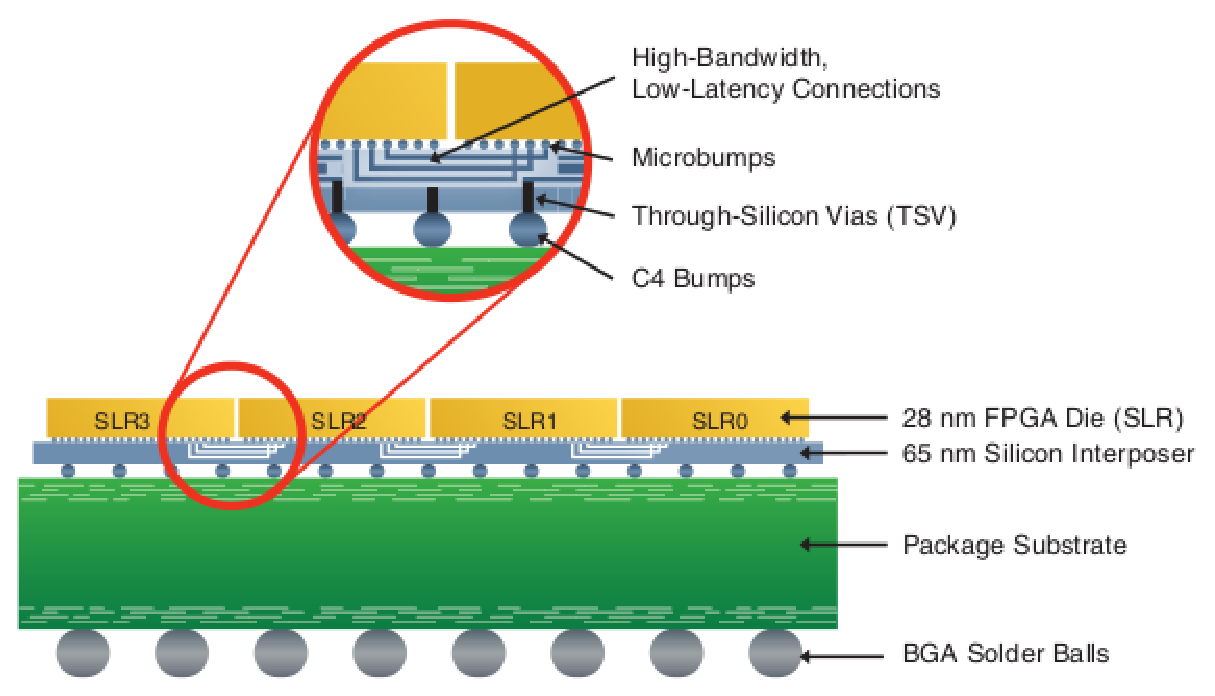
\includegraphics[width=\linewidth]{interposer.eps}
\caption{Lateral view of an interposer-based FPGA\cite{xilinxWP}. The FPGA dice are at the top, and are connected to the silicon interposer through microbumps. The interposer is then connected to the substrate through C4 bumps.}
\label{fig:interposer}
\end{figure}

% Xilinx details:
%  -> 13440 wires crossing
%  -> ~63k vertical wires
%  -> Micro-bumps -> pitch is 45um
%  -> Spread out near edge, to get more bumps
%  -> But results in longer signal travel
%  -> Net result: more delay, reduced connectivity

The \textit{XC7V2000T} is composed of four identical dice arranged such that the vertical routing crosses between the dice. Each horizontal edge of each die has 280 groups of 48 length-12 wires crossing the interposer, which sums to a total of 13440 wires between dice. There are also 40 clock wires crossing the interposer. The average number of wires per vertical channel of this FPGA is 210 and there are approximately 280 vertical channels on the FPGA, resulting in approximately 58800 vertical wires crossing a horizontal cutline within a die. Hence the number of wires which cross the interposer is about 23\% of the total number of within-die vertical wires.

The 28nm dies are connected to the 65nm silicon interposer through microbumps with a 45$\mu$m pitch. Hence the area occupied by microbumps at one edge of one die is 13440 $\times$ (45$\mu$m)\textsuperscript{2} $=$ 27mm\textsuperscript{2}. If we assume each die is $7 \times 12 mm$, as presented by Chaware et al. in \cite{xilinxTSV}, the bumps have to be spread out near the edge and need to go as far as $2.25mm$ away from the edge of the die. This greater distance from the border increaes the length of the inter-die connections, and along with the presence of the micro-bumps and their capacitance, leads to an increased delay for these crossing wires vs. that of a typical on-die routing wire. Chaware et al. state that the latency to cross the interposer is approximately $1ns$. For comparison, a typical medium length 28 nm FPGA routing wire (e.g. spanning four logic blocks) has a delay of approximately 125 ps, while a longer wire (e.g. spanning 12 logic blocks) has a delay of approximately 250 ps.

Overall, these interposer-based FPGAs have increased delay and reduced connectivity between dies, with approximately $23\%$ of the usual number of vertical wires crossing between dies and approximately $1ns$ of increased delay to cross the interposer.

\section{Architecture models}
\label{archSection}
%   - Define parameters
To properly model a silicon interposer FPGA, the popular FPGA exploration toolset, Verilog-to-Routing (VTR)~\cite{vtr2012}, was used. The logic synthesis portions of the flow (ODIN II and  ABC) were left untouched, while the placement and routing portion of the flow (VPR~\cite{betz1997vpr}) was modified to model and optimize for interposer-based FPGAs. The modifications were made in such a way that they require no changes to any of the input files, so one can experiment with interposer-based FPGAs with any existing benchmark circuits and any existing VPR-format FPGA architecture description simply by specifying appropriate command-line parameters.

Three parameters were added to VPR: \textit{\% wires cut}, \textit{increased delay} and \textit{number of cuts}. These three parameters describe the interposer portion of the 2.5D FPGA as detailed below.

%   - % wires cut
\subsection{\% wires cut}
This variable describes and models the reduced connectivity between different dice by specifying the fraction of routing wires that are removed at the border between dice. For example, if a channel had 200 wires and \textit{\% wires cut} was 70, 140 of them would be cut and only 60 would pass through the interposer. Higher values of \textit{\% wires cut} make an interposer easier to manufacture, and can reduce the interposer delay by allowing all the microbumps linking dice to be placed near the die edge. However, the higher \textit{\% wires cut} is, the less routable the multi-die system becomes. As described in \ref{virtex7section}, the Virtex 7 family has \textit{\% wires cut} $=$ 77\%.

%   - Added delay
\subsection{Increased delay}
Interposer wires are longer and wider than on-die wires and have microbumps on each end. \textit{Increased delay} models the resulting larger delay when compared with wires which are internal to a die. A reasonable estimate for this variable is around $1ns$, as presented by Chaware et al\cite{xilinxTSV}.

%	- number of cuts
\subsection{Number of cuts}
\textit{Number of cuts} describes how many cuts were made to the interposer-based FPGA versus a monolithic die. If \textit{number of cuts} equals 1 then there are 2 dies, and so on. We investigate values of this parameter between 1 and 3 (between 2 and 4 dies), reflecting commercial practice: the Virtex 7 family has members with \textit{number of cuts} $=$ 2 and 3. Figure \ref{fig:fpga} shows a sample architecture with one cutline.

\begin{figure}[!htbp]
\centering
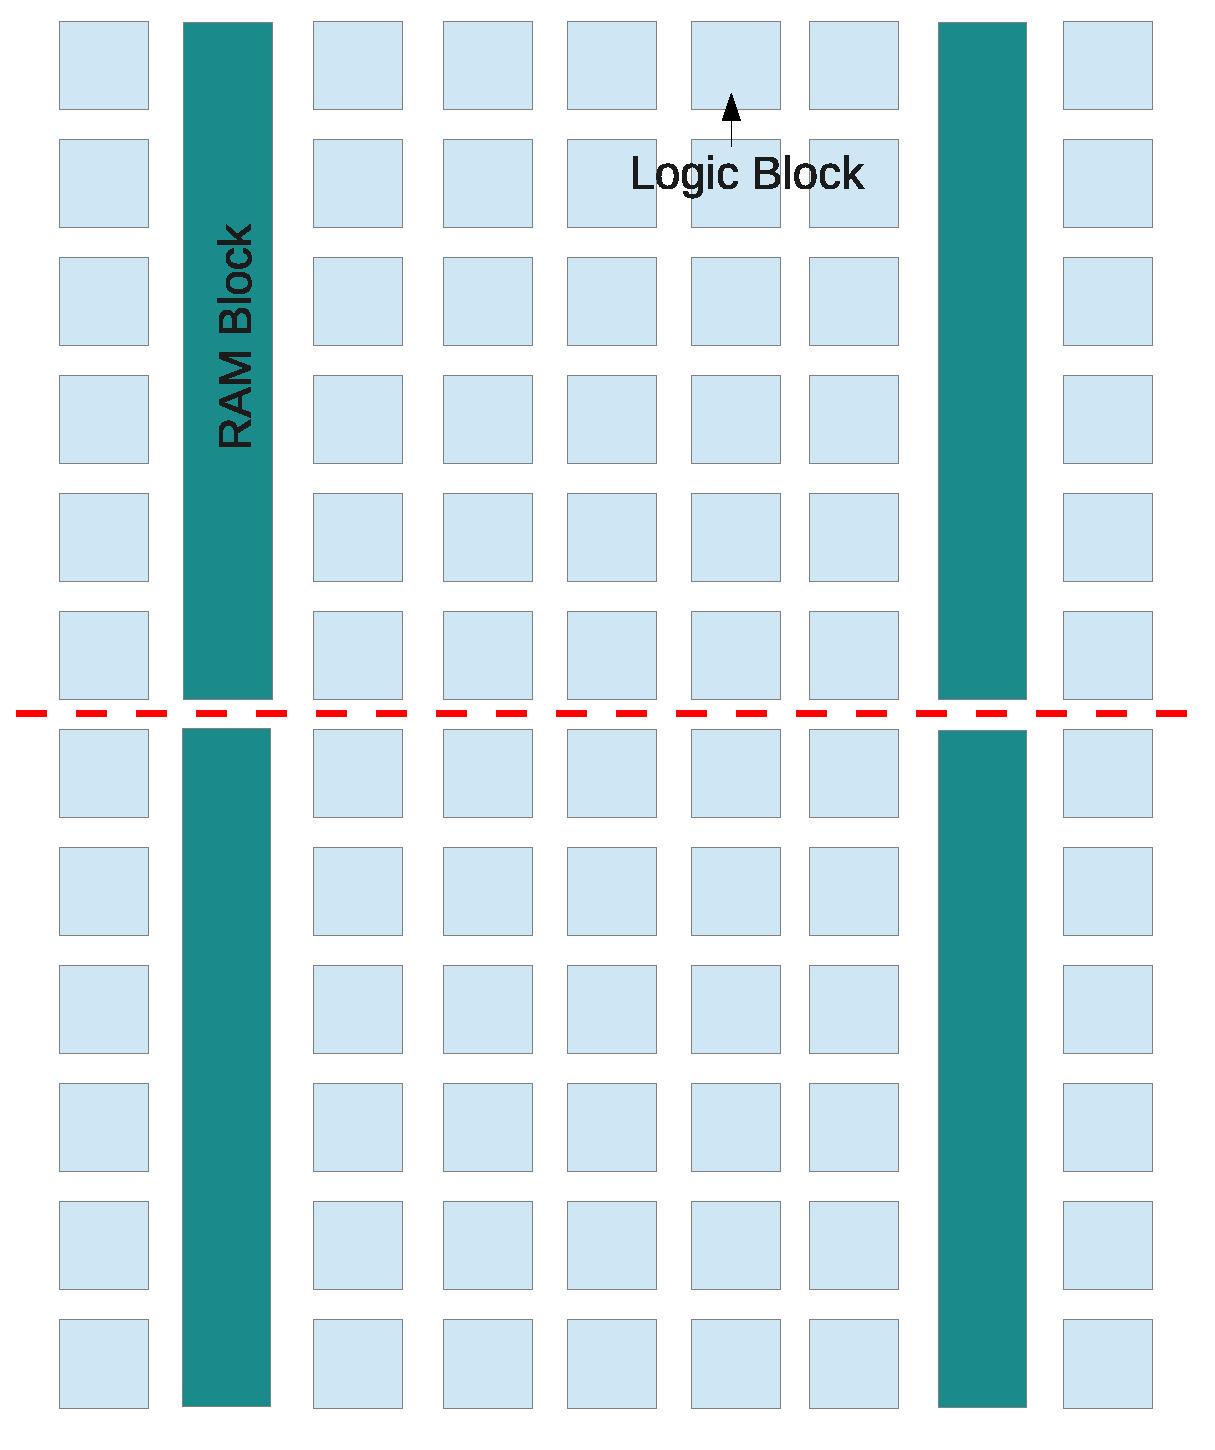
\includegraphics[width=\linewidth]{fpga.eps}
\caption{A sample two-die / 1-cutline architecture containing both logic blocks and RAM blocks.}
\label{fig:fpga}
\end{figure}

%   - (briefly) explain how it was put in VPR
\subsection{Implementation}
To model an interposer-based FPGA in VPR the Routing Resource Graph (\textit{rrgraph}) must be modified. The rrgraph is the data structure that defines all the available routing wires and switches in the FPGA, as well the delay of each. Given a suitable rrgraph, the VPR router can implement circuits in the desired FPGA, and the VPR timing analyzer can estimate their delay.

The presence of multiple dice in an interposer-based FPGA was modeled by creating horizontal cuts in the FPGA, which are equally spaced vertically. Every wire that crosses one of these cuts in fact passes through the interposer. In the experiments below, we use an architecture that has only unidirectional wires~\cite{unidirectional}, as these are the dominant routing architecture in modern FPGAs. Such wires can only be driven at their beginning. To control the wiring capacity between dies \textit{\% wires cut} wires of each channel segment crossing a cutline have their connections to wires and block inputs on the die opposite to their starting point removed, and the wires which aren't cut have \textit{increased delay} added to their connections which cross the cutline. Note that the combination of a unidirectional routing architecture and a silicon interposer results in some blocks near the cutline having reduced routing connectivity as some of the routing wires driving their inputs are disconnected from the (single) wire driver, when that driver is on the other side of the cutline and the wire is one of the cut wires.

Figure \ref{fig:implementation} illustrates the approach used.

\begin{figure}[!htbp]
\centering
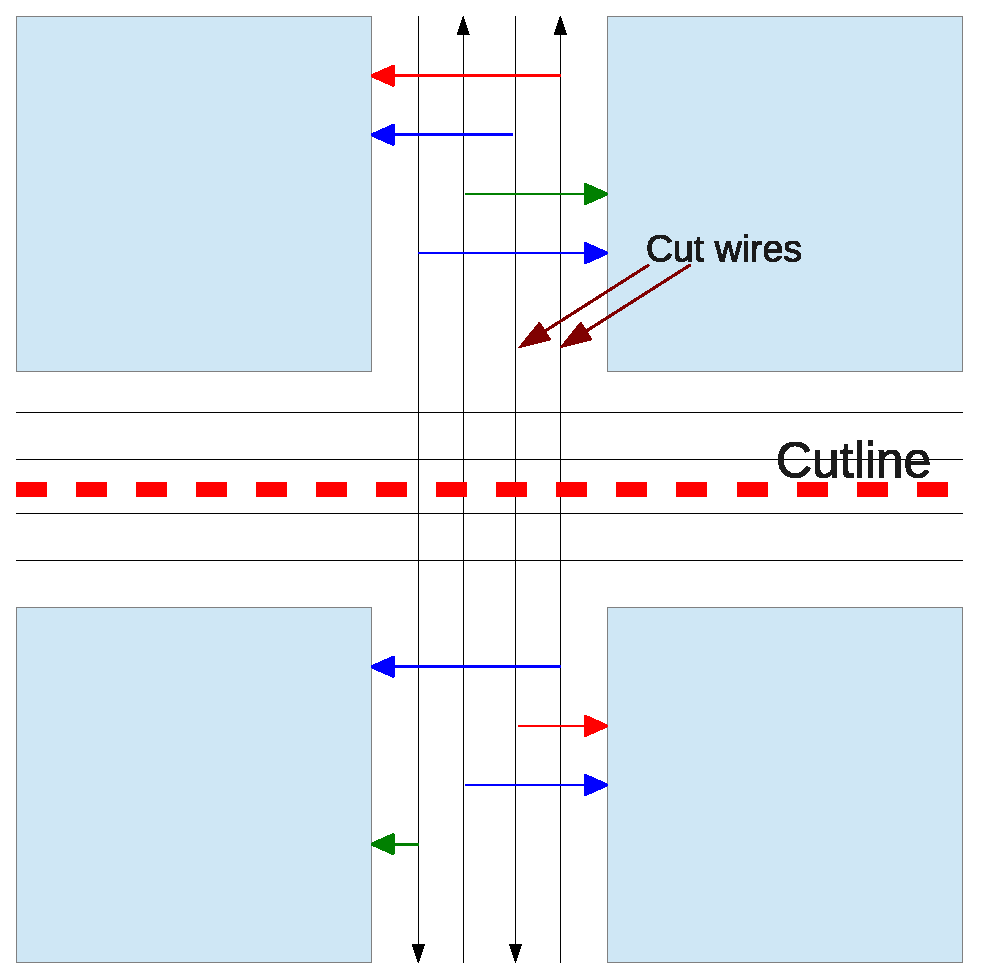
\includegraphics[width=\linewidth]{implementation.eps}
\caption{Illustration of the approach used to simulate crossing the interposer. The red dashed line indicates the interposer, the black arrows indicate the direction of the wires. Blue arrows indicate normal connections from the wires to the CLBs. The red arrows indicate removed connections and green arrows indicate connections with increased delay.}
\label{fig:implementation}
\end{figure}

For all experiments in this paper, the remaining architecture parameters of the FPGA are taken from the "flagship" architecture of the VTR project (\textit{k6\_frac\_N10\_mem32K\_40nm.xml}). The parameters of this architecture are in line with both current commercial FPGAs and academic research into best practices. It consists of logic clusters with 10 fracturable 6-LUTs per block (N=10, k=6), and also includes 32kb RAM blocks and DSP blocks configurable to perform 9x9, 18x18 or 36x36 multipliers. The delay values in the architecture are taken from 40 nm circuit simulations and 40 nm commercial FPGAs. It uses unidirectional routing, with all wire segments having length L = 4.

\section{CAD Enhancements}
\label{cadSection}

Once the routing resource graph was modified as detailed in Section \ref{archSection}, the VPR router adapted automatically to the interposer architecture. Placement, however, is crucial in mitigating the impact of the reduced wiring and increased delay when crossing between dice; a good placement should minimize the number of signals crossing between dice, particularly time-critical ones. We investigated several enhancements to VPR's placement cost function to improve result quality. 

VPR uses 2 different costs as the metrics for its placer algorithm: the timing cost and the bounding box (wiring) cost. The usual VPR timing cost is a (criticality-weighted) summation of the estimated delay (given the current placement) of every connection required by the circuit~\cite{timing2000}:

\begin{equation} \label{eq:timing_eq_full}
\begin{split}
Timing\_Cost = \sum_{\forall i, j \subset circuit} delay(\Delta x_{ij},\Delta y_{ij}) \times \\ 
criticality(i,j)
\end{split}
\end{equation}

where \textit{ij} denotes a connection from block i to block j that exists in the circuit netlist.
The bounding box cost estimates the amount of wiring required for a net, based on the number of pins and size of the net's bounding box. VPR's original formulation is~\cite{betz1997vpr}:

\begin{equation} \label{eq:bbcost}
\begin{split}
wiring\_cost_{orig} = \sum_{n=1}^{N_{nets}} q(n) \times [\frac{bb_x(n)}{avg\_chanx\_W(n)} + \\
\frac{bb_y(n)}{avg\_chany\_W(n)}]
\end{split}
\end{equation}

where $bb_x(n)$ and $bb_y(n)$ are the dimensions of the bounding box of net \textit{n} in the x and y directions, respectively. $avg\_chanx\_W$ and $avg\_chany\_W$ are the average x-directed and y-directed channel widths over this bounding box. Finally, $q(n)$ is a function obtained from \cite{icann} which models the fact that bounding boxes underpredict the required routing for high fanout nets. $q(n)$ slowly increases with the fanout of net \textit{n}, rising from 1 for nets with 3 or fewer terminals to 2.79 for nets with 50 terminals.

We modified both the placer's bounding box and timing costs to account for the increased latency to cross the interposer and for the reduced wire capacity close to the cutlines, as the wire availability becomes more sparse.

%   - Delay
\subsection{Placer timing cost}
The standard placer timing cost in VPR assumes that the FPGA is homogeneous and consequently the delay between 2 points $(x_1,y_1)$ and $(x_2,y_2)$ only depends on $(\Delta x,\Delta y)$. This is obviously not true for interposer-based FPGAs, as the cutlines make them heterogeneous in the \textit{y} direction.

To solve this problem and improve the quality of the results, an extra term was added to the delay function. The delay function becomes:

\begin{equation} \label{eq:timing_cost}
\begin{split}
delay(i,j) =& delay(\Delta x_{ij}, \Delta y_{ij}) + \\
&times\_crossed(i,j) \times delay\_increase
\end{split}
\end{equation}

where $times\_crossed(i,j)$ is the number of times this path has to cross the interposer to go from $(x_i,y_i)$ to $(x_j,y_j)$ and $delay\_increase$ is the timing penalty of crossing the interposer.

%   - Wiring / cut cost
\subsection{Placer wiring cost}
VPR's wiring cost also considers the FPGA to be homogeneous, and uses only the number of nets, the size of the net's bounding box and the average number of wires per channel to calculate the cost. Thus, to account for the reduced connectivity near the cutlines an extra cost term, \textit{cut\_cost}, was created. This new cost is added to (\ref{eq:bbcost}) to create the total wiring cost.

\begin{equation} \label{eq:total_wiring}
wiring\_cost = wiring\_cost_{orig} + cut\_cost
\end{equation}

We tested several different \textit{cut\_cost} formulations, as well as different weighting (C values) for each. For all of the formulations the variable $C'$ was defined as:

\begin{equation} \label{eq:cprime}
\begin{split}
C' = \frac{C \times ratio\_wires\_cut}{avg\_chany\_W(n)}
\end{split}
\end{equation}

where $ratio\_wires\_cut$ is the ratio of wires cut at the cutline. This formulation of $C'$ ensures that when we choose a \textit{C} value of 1, the new term cost term is of roughly the same magnitude as $wire\_cost_{orig}$ in (\ref{eq:bbcost}) and that it is weighted more heavily for interposer architectures in which the wiring between dice is more scarce.

The first \textit{cut\_cost} term we tested was:

\begin{equation} \label{eq:cost0}
cut\_cost = \sum_{n=1}^{N_{nets}} C' \times times\_crossed(n)
\end{equation}

which penalizes the net according to the number of cutlines the bounding box spans; this directly penalizes each signal crossing between dice. Surprisingly this extra term did not result in significant improvements to the quality of results and in some cases even made them worse. We believe this is due to the discontinuous, non-smooth, nature of this cost function -- it does not guide placement optimization well as a bounding box shrinks toward a cutline. Placement changes that make bounding boxes "almost not cross" a cutline are not given any gain; only a sudden change in the placement that moves a bounding box entirely to one side or the other of the cutline yields a cost reduction. This insight led us to the other proposed functions, which give gradual gains as bounding boxes change in their size and come closer to avoiding a cutline crossing.

The other tested terms were:

%add C' x times_crossed(i)

\begin{equation} \label{eq:cost1}
cut\_cost = \sum_{n=1}^{N_{nets}} C' \times bbWidth(n) \times times\_crossed(n)
\end{equation}

\begin{equation} \label{eq:cost2}
cut\_cost = \sum_{n=1}^{N_{nets}} C' \times bbHeight(i) \times times\_crossed(n)
\end{equation}

\begin{equation} \label{eq:cost4}
\begin{split}
cut\_cost = \sum_{n=1}^{N_{nets}} C' \times minDist(i) \times times\_crossed(n) +\\
C' \times times\_crossed(n)
\end{split}
\end{equation}

\begin{equation} \label{eq:cost5}
cut\_cost = \sum_{n=1}^{N_{nets}} C' \times bbHeight(n)
\end{equation}

where \textit{bbWidth(n)} and \textit{bbHeight(n)} are the width and height of the bounding box of the net \textit{n}, respectively, and \textit{minDist(n)} is the minimum distance from the top or bottom of the bounding box to a cutline. 

%   - Effectiveness / results
\subsection{Effectiveness of the enhancements}
\label{sec:CADeffect}

We used VPR 7.0, with the enhancements we detailed above, and the architecture file \textit{k6\_frac\_N10\_mem32K\_40nm} in the experiments below. All experiments targeted the smallest FPGA (with number of rows equal to number of columns) which could accomodate a benchmark circuit; this represents a very full FPGA with little white space left, and hence presents a difficult case to an interposer-based FPGA as no die can be left mostly empty.

Figures \ref{fig:minW_constant_sweep} and \ref{fig:areadelay_constant_sweep} show the efficacy of the five placer wiring cost modifications as their weight, \textit{C} varies. Each point in the graphs is the geometric mean of the results with \textit{\% wires cut} = 60 and 80, and the results for 60\% and 80\% are themselves geometric means of the results of 6 circuits from the VTR benchmark suite~\cite{vtr2012}:  \textit{stereovision0}, \textit{stereovision1}, \textit{mkDelayWorker32B}, \textit{mkSMAdapter4B}, \textit{or1200} and \textit{blob\_merge}. These values for \textit{\% wires cut} were chosen because they in the likely range of wires which can cross the interposer without exceeding the microbump capacity, as described in Section~\ref{virtex7section}. The \textit{area-delay product} is the product of the \textit{minimum channel width} and the \textit{critical path delay}. To obtain the \textit{critical path delay} the circuits were run with a low stress routing with a channel width, $W = 1.3 \times minW$, where $minW$ is the minimum channel width for which the circuit is still routable. 

\begin{figure}[!htbp]
\centering
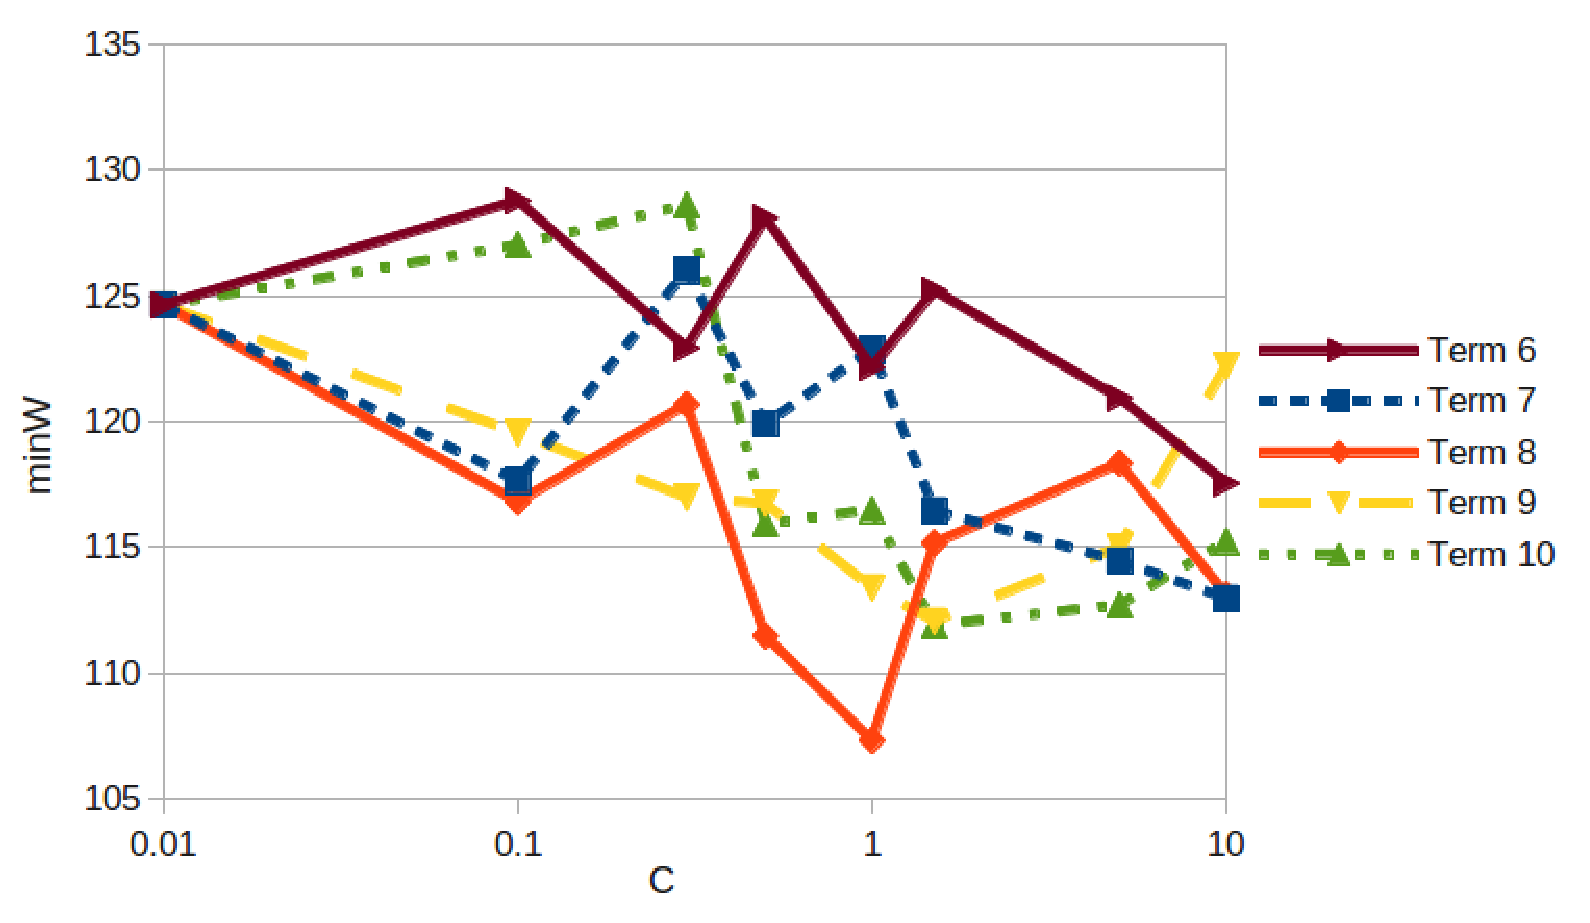
\includegraphics[width=\linewidth]{minW_constant_sweep_log.eps}
\caption{Minimum channel width vs. weighting for different \textit{cut\_cost} terms.}
\label{fig:minW_constant_sweep}
\end{figure}

\begin{figure}[!htbp]
\centering
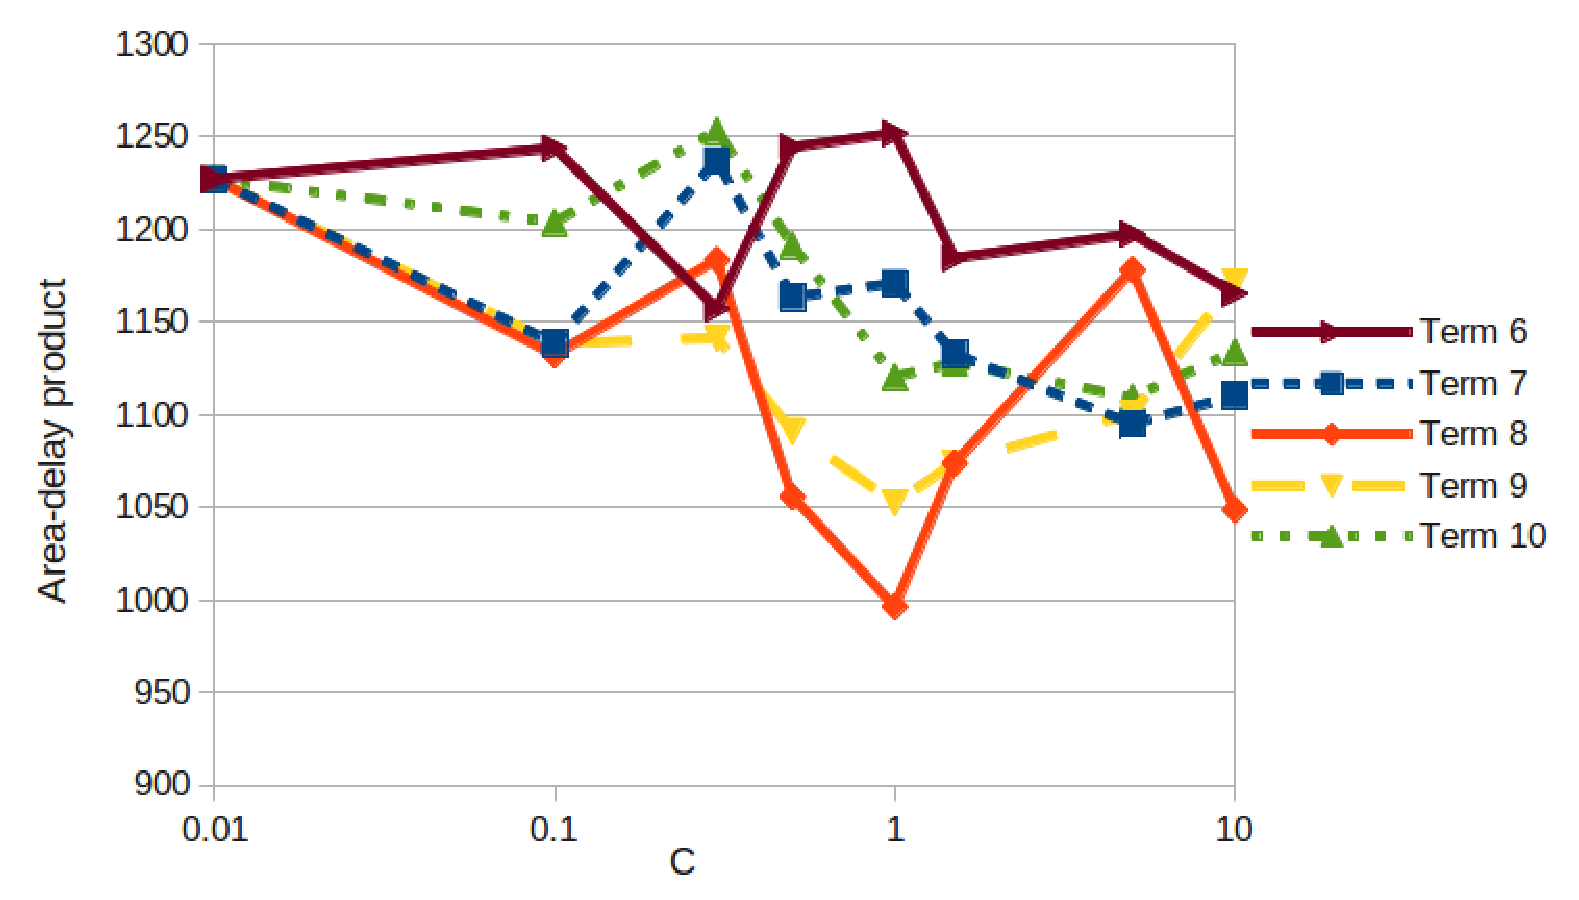
\includegraphics[width=\linewidth]{areadelay_constant_sweep_log.eps}
\caption{Area-delay product vs. weighting for different \textit{cut\_cost} terms.}
\label{fig:areadelay_constant_sweep}
\end{figure}

\begin{table}[htbp]
\begin{tabular}{|r|r|r|r|r|}
\hline
\multicolumn{1}{|l|}{Term} & \multicolumn{1}{l|}{Best C} & \multicolumn{1}{l|}{minW} & \multicolumn{1}{l|}{crit\_path(ns)} & \multicolumn{1}{l|}{Area-delay} \\ \hline \hline
None & - & 124.636 & 9.844 & 1226.955 \\ \hline
\ref{eq:cost0} & 0.3 & 122.929 & 9.413 & 1157.09 \\ \hline
\ref{eq:cost1} & 5 & 114.444 & 9.565 & 1094.68 \\ \hline
\ref{eq:cost2} & 1 & 107.303 & 9.285 & 996.26 \\ \hline
\ref{eq:cost4} & 1 & 113.381 & 9.280 & 1052.16 \\ \hline
\ref{eq:cost5} & 5 & 112.703 & 9.841 & 1109.11 \\ \hline
\end{tabular}
\caption{Best weighting and performance for each \textit{cut\_cost} term.}
\label{table:constant_sweep}
\end{table}

The best \textit{C} value and the resulting performance for each term is summarized in Table~\ref{table:constant_sweep}. Note that cost term (\ref{eq:cost2}) with weighting $C = 1.0$ has the best performance; this is the configuration used in the rest of our experiments.

We believe the key to the good performance of this cost function is that it produces gradual gains as bounding boxes crossing the cutline shrink to be closer and closer to being captured entirely on one side of the cutline. Consider for example the 3 bounding boxes shown in Figure \ref{fig:bb_illustration}. Note that bounding box (a) and (b) both cross the cutline and hence are penalized equally by (\ref{eq:cost0}), while bounding box (c) does not cross a cutline and hence is not penalized. However, bounding box (b) is mostly on the lower side of the cutline; it is more likely that later smaller placement changes will result in the bounding box moving entirely below the cutline, reducing interposer wiring demand. Cost function terms (\ref{eq:cost2}) and (\ref{eq:cost4}) will both penalize bounding box (a) more than bounding box (b) to guide placement to gradually move bounding boxes to one side or the other of a cutline. Figure \ref{fig:areadelay_constant_sweep} shows that these are the two best performing \textit{cut\_cost} terms.

\begin{figure}[!htbp]
\centering
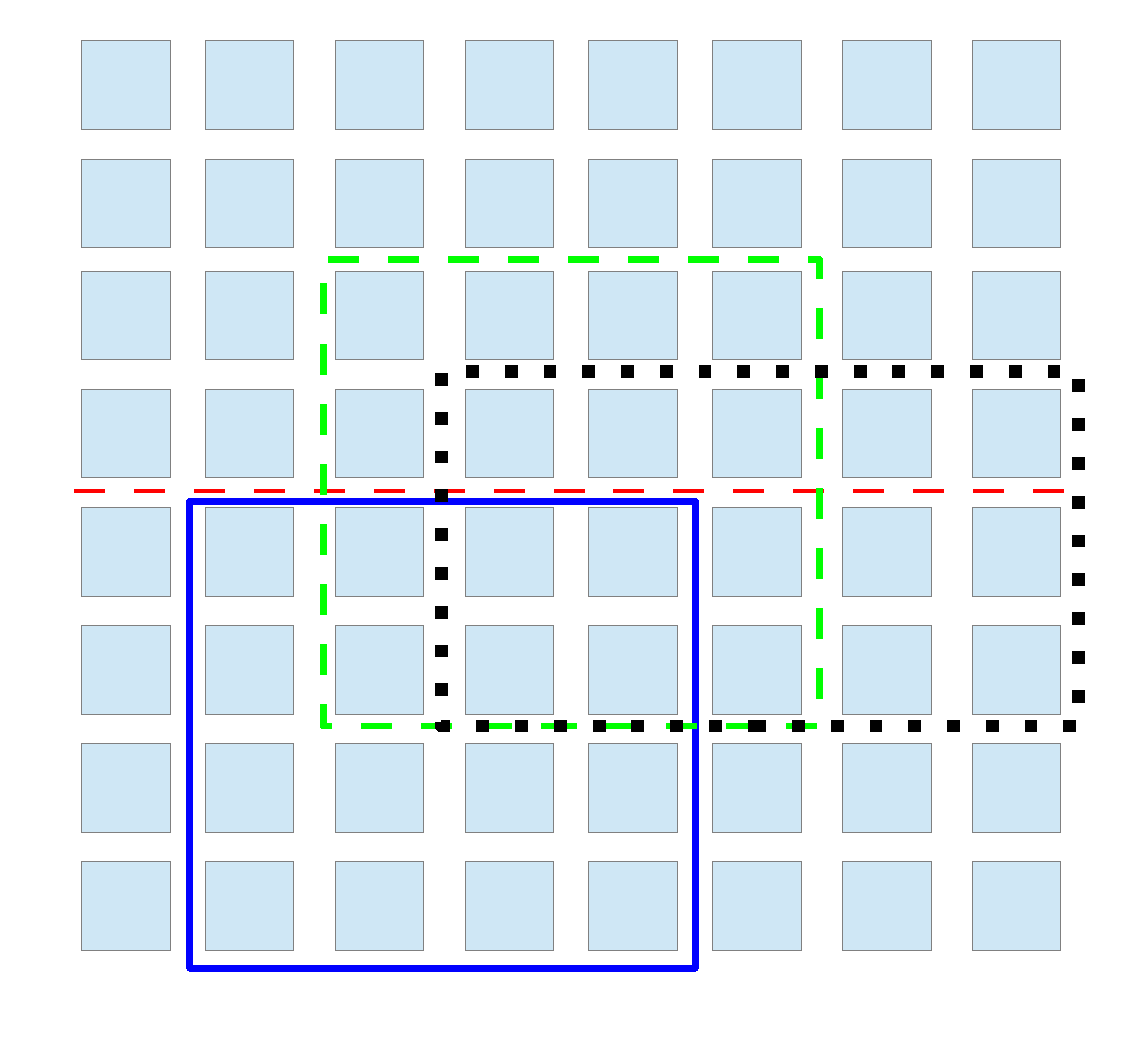
\includegraphics[width=\linewidth]{bb.eps}
\caption{Illustration of three different scenarios for the wiring cost. The dashed green box shows a case where \textit{(a)} it crosses the interposer, the dotted black box shows a case where \textit{(b)} it barely crosses the cutline, and the solid blue one shows a case where \textit{(c)} the bounding box does not span the cutline.}
\label{fig:bb_illustration}
\end{figure}

Figure \ref{fig:comparison_minW} shows the minimum channel width for different values of \textit{\% wires cut} when there are no optimizations and when \textit{cut\_const} (\ref{eq:cost2}) is used. % comment about impact vs % wires cut
Figure \ref{fig:comparison_bars} compares result quality with both enhanced timing and wiring cost functions. These experiments were run with term (\ref{eq:cost2}), and are the geometric means of the runs with \textit{\% wires cut = 60, 70, 80}. 

\begin{figure}[!htbp]
\centering
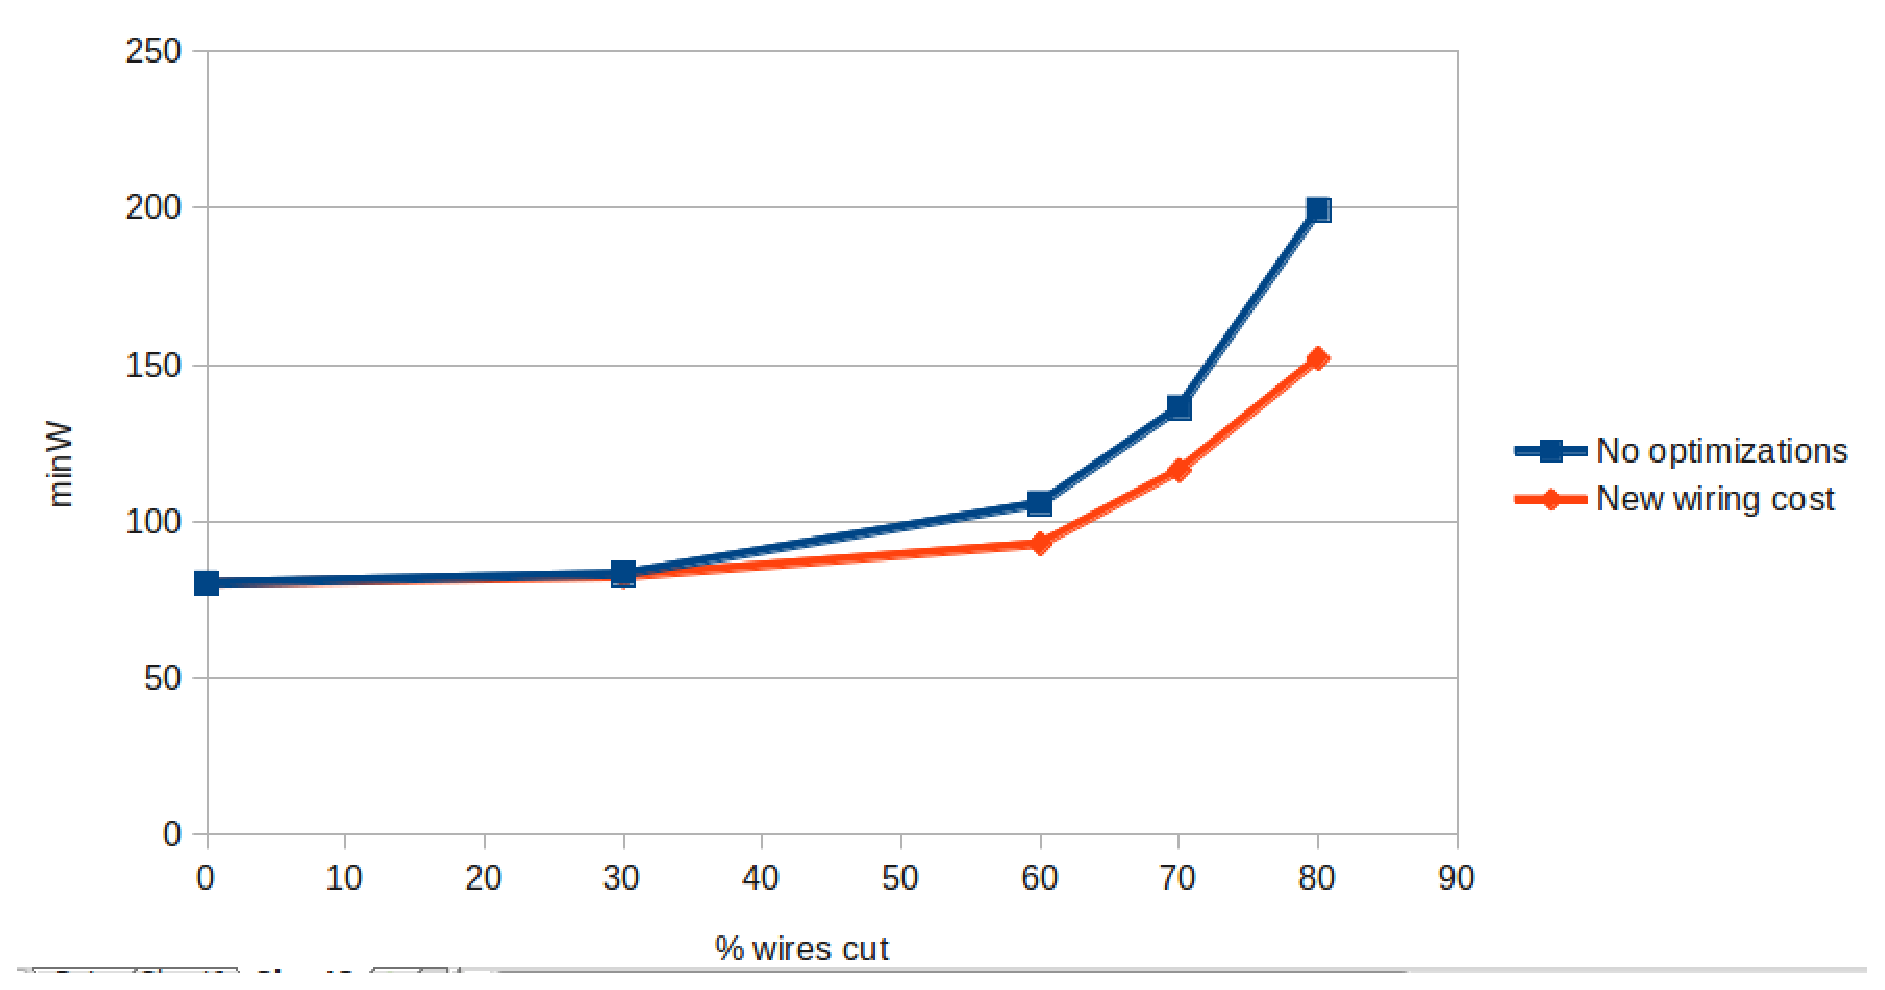
\includegraphics[width=\linewidth]{comparison_minW.eps}
\caption{Minimum channel width vs. \textit{\% wires cut}.}
\label{fig:comparison_minW}
\end{figure}

\begin{figure}[!htbp]
\centering
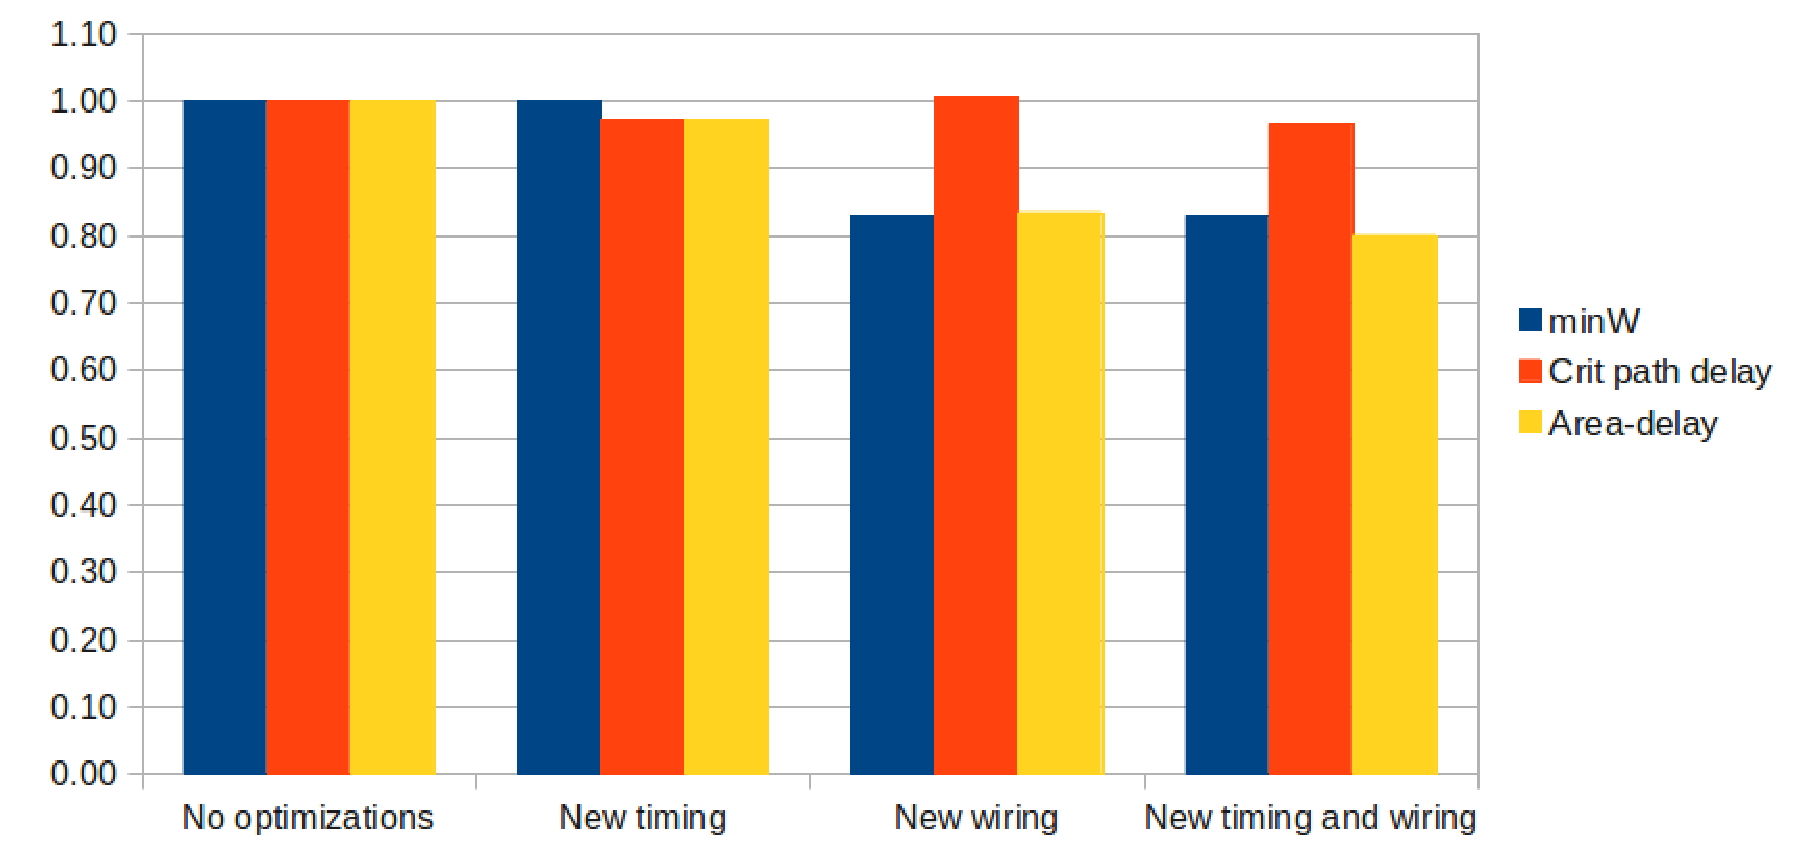
\includegraphics[width=\linewidth]{comparison_bars_relative.eps}
\caption{Performance of different placer optimizations, relative to the original VPR results. The area-delay product is calculated as the product $minW \times critical path delay.$}
\label{fig:comparison_bars}
\end{figure}

The graphs show that combining the timing with the bounding box optimizations led to an average of 20\% improvement on the area-delay product and the most significant contribution was made by incorporation of \textit{cut\_cost} into the wire cost function.


%----------------------------------------------------
\section{Architecture results}
\label{resultsSection}

Using the best CAD settings found in Section~\ref{cadSection} we analyzed the impact of three key architecture parameters:  \textit{\% wires cut}, \textit{delay increase} and \textit{number of cuts}. All the experiments were run with the eight largest circuits from the VTR benchmark~\cite{vtr2012}, namely: \textit{bgm}, \textit{LU8PEEng}, \textit{LU32PEEng}, \textit{mcml}, \textit{mkDelayWorker32B}, \textit{stereovision0}, \textit{stereovision1} and \textit{stereovision2}. The size of these circuits ranges from $9,100$ to $153,000$ primitives (LUTs, FFs, etc.), with an average size of $52,600$ primitives. All results are the geometric mean over all circuits for a given interposer architecture.

%   - Channel width vs % wires cut
\subsection{Interposer Wiring Capacity (\% wires cut)}

To analyze the impact of the number of cut wires we ran experiments varying only this parameter while leaving the number of cuts and the increased delay constant. The values used for these parameters were \textit{number of cuts} $= 3$ (corresponding to four dice) and \textit{increased delay} $= 1ns$, as these values are similar to those of the \textit{XC7V2000T} device.

Figure \ref{fig:standard_minW} shows the graph of minimum channel width versus \textit{\% wires cut}. It can be noted from this graph that the minimum channel width increases slowly up to 60\% of wires cut, indicating that the placement engine is able to avoid saturating the interposer routing until that point. When more than 60\% of the wires are cut however (i.e. the interposer provides less than 40\% of the usual within-die routing capacity), the minimum channel width grows rapidly indicating that the interposer routing bandwidth has become a limiting factor. The minW value at 60\% is 20\% greater than with no wires cut, while at 70\% it is 52\% above and at 80\% it is 125\% larger than the minW with no cut wires.

The critical path delay, depicted in Figure~\ref{fig:standard_crit}, on the other hand, is not strongly influenced by the percentage of wires cut, as the critical path delay at 60\% of the wires cut is essentially the same as at 0\% wires cut. At 80\% of the wires cut the critical path delay does rise somewhat, by 6\%; this is due to two factors: the placement is being modified to improve routability at the expense of timing, and some circuitous routes are occuring due to saturated interconnect across the interposer.
%Andre, what is the critical path delay with no interposer (i.e. 0% cut and 0 delay)?

Tables \ref{table:standard_minW} and \ref{table:standard_path} show the minimum channel width and critical path delay for each circuit. The trends for individual circuits follow those of the averages quite closely.

\begin{figure}[!htbp]
\centering
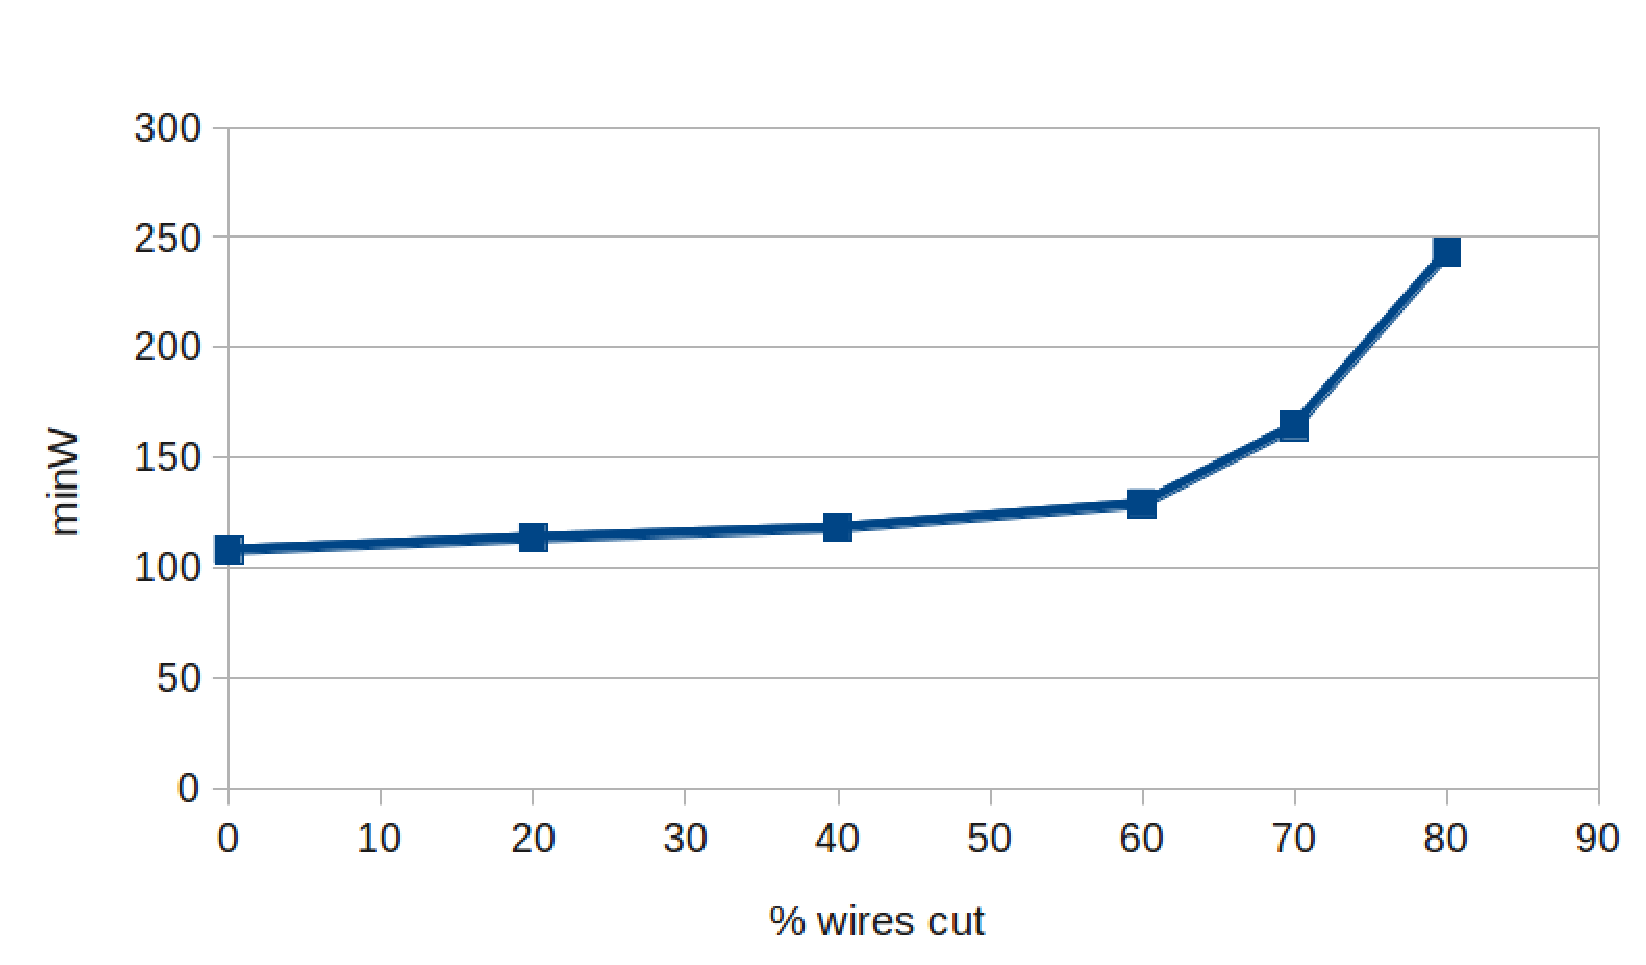
\includegraphics[width=\linewidth]{standard_minW.eps}
\caption{Minimum channel width vs. \textit{\% wires cut} for 3 cuts and $1ns$ of \textit{delay increase}.}
\label{fig:standard_minW}
\end{figure}

\begin{figure}[!htbp]
\centering
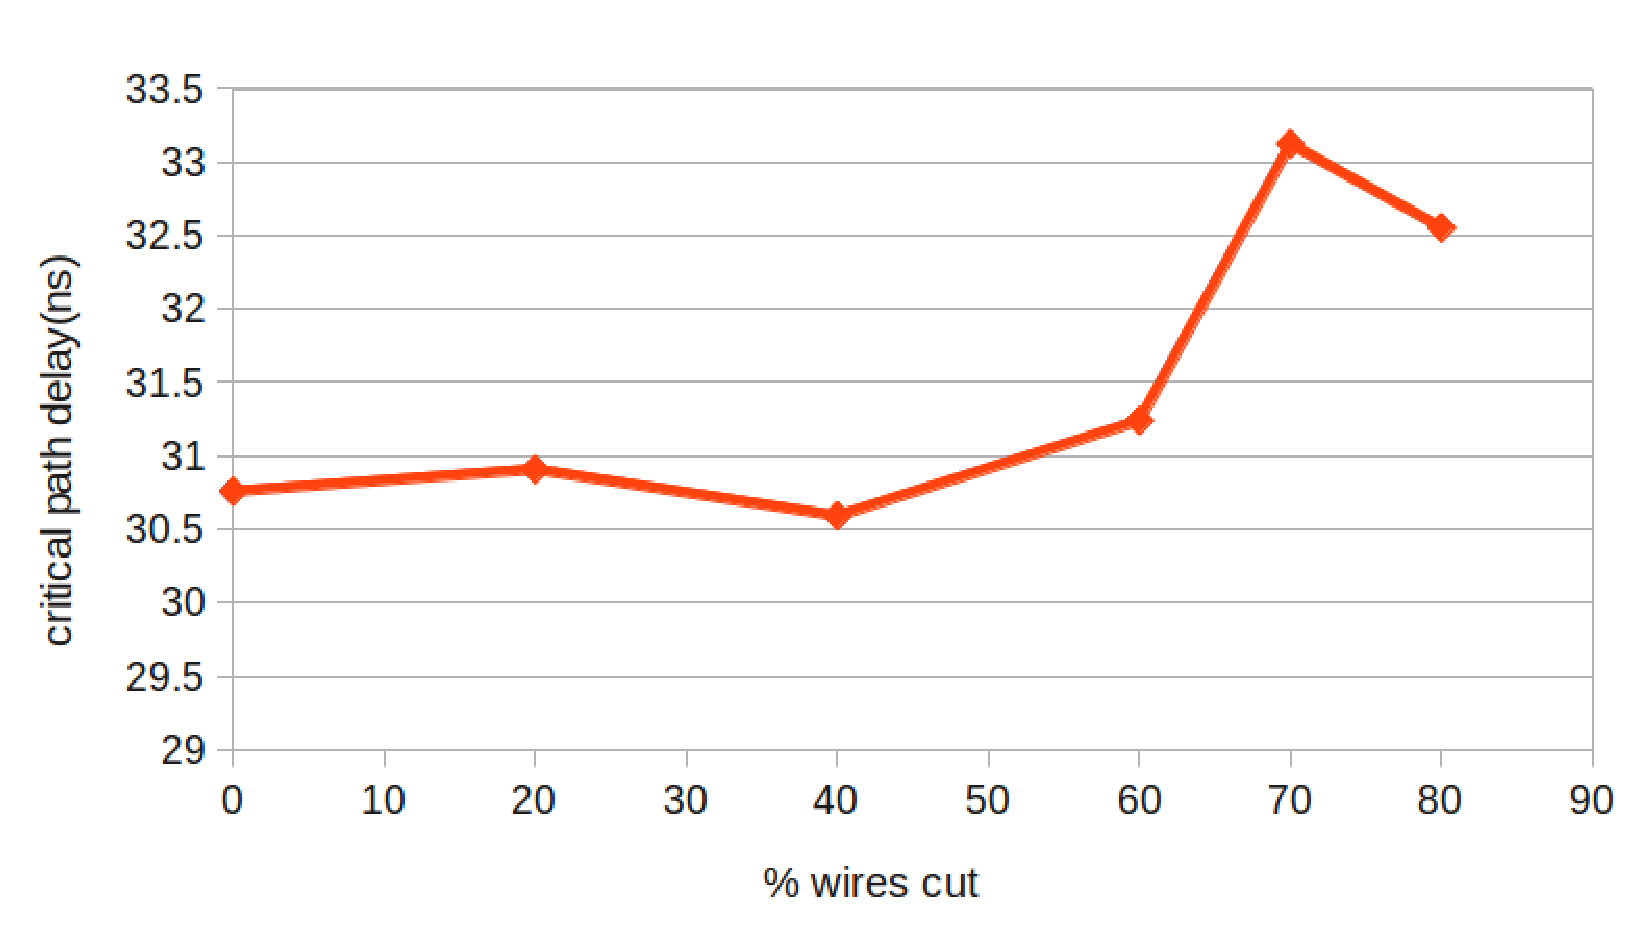
\includegraphics[width=\linewidth]{standard_crit_path.eps}
\caption{Critical path delay vs. \textit{\% wires cut} for 3 cuts and $1ns$ of \textit{delay increase}.}
\label{fig:standard_crit}
\end{figure}

\begin{table}[!htbp]
\begin{tabular}{|l|r|r|r|r|r|r|}
\hline
\% wires cut & 0 & 20 & 40 & 60 & 70 & 80 \\ \hline \hline
bgm & 114 & 128 & 124 & 132 & 152 & 226 \\ \hline
LU32PEEng & 172 & 178 & 182 & 218 & 304 & 426 \\ \hline
LU8PEEng & 110 & 116 & 118 & 128 & 158 & 236 \\ \hline
mcml & 108 & 124 & 128 & 116 & 152 & 218 \\ \hline
mkDelayWorker32B & 76 & 80 & 82 & 88 & 100 & 132 \\ \hline
stereovision0 & 62 & 60 & 70 & 88 & 110 & 166 \\ \hline
stereovision1 & 104 & 108 & 116 & 120 & 178 & 312 \\ \hline
stereovision2 & 162 & 164 & 168 & 194 & 244 & 360 \\ \hline
Geometric mean & 108 & 114 & 118 & 129 & 164 & 243 \\ \hline
\end{tabular}
\caption{Minimum channel width when \textit{number of cuts = 3} and \textit{increased delay = 1ns}.}
\label{table:standard_minW}
\end{table}

\begin{table}[!htbp]
\begin{tabular}{|l|r|r|r|r|r|r|}
\hline
\% wires cut & 0 & 20 & 40 & 60 & 70 & 80 \\ \hline \hline
bgm & 35.1 & 33.6 & 32.2 & 32.9 & 37.8 & 40.3 \\ \hline
LU32PEEng & 115 & 114 & 114 & 114 & 115 & 113 \\ \hline
LU8PEEng & 118 & 117 & 119 & 116 & 117 & 124 \\ \hline
mcml & 82.3 & 82.9 & 84.0 & 83.4 & 88.3 & 85.7 \\ \hline
mkDelayWorker32B & 11.0 & 12.3 & 12.0 & 12.3 & 14.4 & 12.8 \\ \hline
stereovision0 & 6.9 & 7.8 & 7.0 & 7.4 & 7.6 & 7.0 \\ \hline
stereovision1 & 11.6 & 9.2 & 10.4 & 11.0 & 11.6 & 11.8 \\ \hline
stereovision2 & 23.3 & 25.4 & 23.9 & 24.9 & 25.6 & 24.8 \\ \hline
Geometric mean & 30.8 & 30.9 & 30.6 & 31.2 & 33.1 & 32.6 \\ \hline
\end{tabular}
\caption{Critical path delay (in \textit{ns}) when \textit{number of cuts = 3} and \textit{increased delay = 1ns}.}
\label{table:standard_path}
\end{table}

% TODO
% "extra FPGA routing channel width" vs. wires across the interposer
%\subsection{Intra-FPGA Routing  width vs. wires across the interposer}

%Can you take a crack at adding a section that tries to present the data as "extra FPGA routing channel width" vs. wires across the interposer?  The idea would be to address reviewer 4's comments:  the graph will show we need some minimum number of wires across the interposer, and it will also directly show how many more wires we need to add to the FPGA to maintain routability.  I think you could get this data simply by processing data you already have.
%So: 
%x-axis:  geomean wires crossing interposer
%y-axis:  geomean channel width required

Figure \ref{fig:crossingwires} provides an alternative way to visualize the relationship between interposer routing supply and routability. This figure shows how the geometric average minimum channel width required within the FPGA dice varies as the geometric average of the \emph{absolute} number of wires crossing the interposer in each channel varies, again for 4-die system. When 108 tracks cross the interposer, the interposer channels have the same capacity as the vertical routing channels within each FPGA die. As fewer wires cross the interposer, the channel width required within the FPGA dice increases to compensate for the routing difficulty in crossing the interposer. The increase is gradual as the interposer routing is reduced from 108 tracks per channel to 52 tracks per channel; over this range the routing per channel required in the FPGA dice increases from 108 tracks per channel to 129 tracks per channel. As the routing crossing the interposer is further reduced however, it becomes very difficult to increase the within-die routing sufficiently to compensate. At 49 tracks crossing the interposer channels, for example, the within-die routing must have a channel width of \emph{243} tracks to successfully route the designs. Clearly the CAD tools have the ability to trade-off interposer routing for within-die routing over a reasonable range but below a certain level (48\% of the original within-die minimum channel width in our experiments) routability becomes almost solely limited by the wiring crossing the interposer and further reduction in interposer routing is not productive.

\begin{figure}[!htbp]
\centering
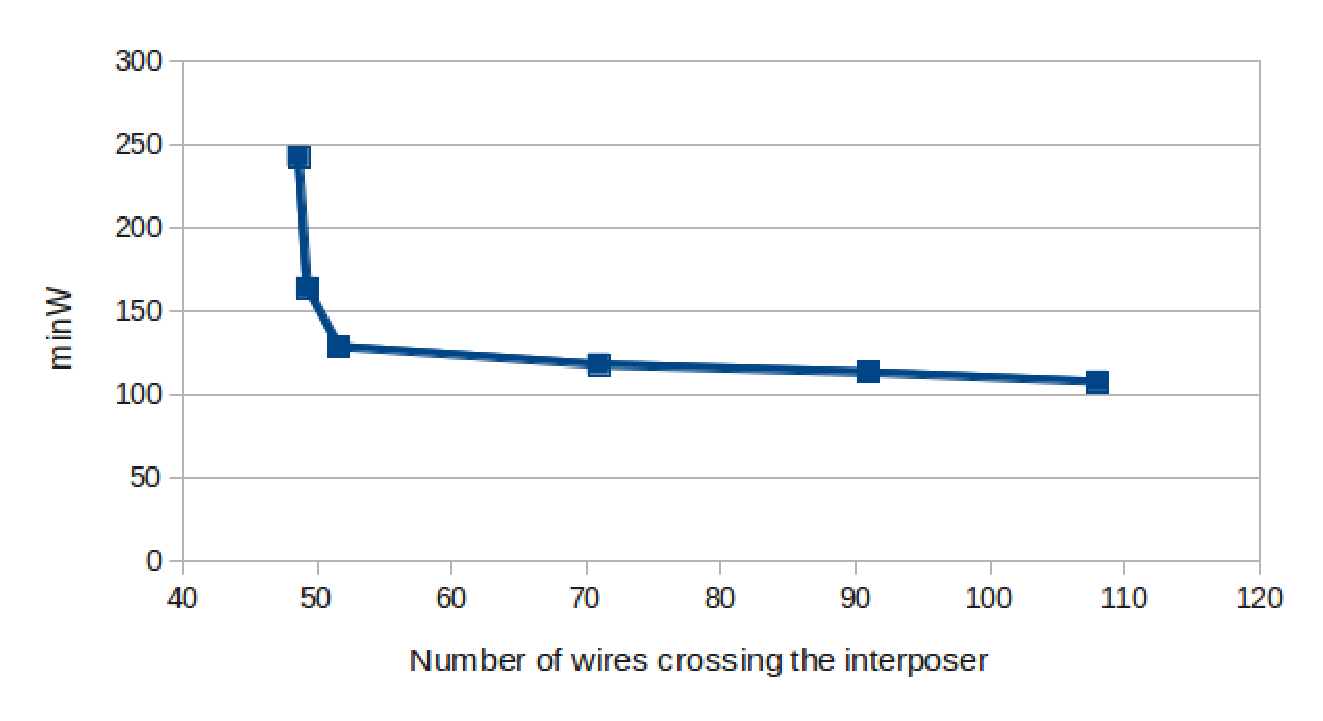
\includegraphics[width=\linewidth]{numberofcrossingwires.eps}
\caption{Geometric mean of required intra-die minimum channel width vs. geometric mean of the number of wires crossing the interposer for 3 cuts and $1ns$ of \textit{delay increase}.}
\label{fig:crossingwires}
\end{figure}

%   - Delay vs % wires cut & wire delay
\subsection{Circuit Speed vs. Interposer Delay}

To investigate the impact of the interposer delay (\textit{delay increase}), we kept the \textit{number of cuts} constant at $3$ while \textit{delay increase} was swept between $0$ and $1.5ns$.

Figure \ref{fig:delays_crit} shows critical path delay versus \textit{\% wires cut} for 4 different values of \textit{delay increase}. The penalty in critical path delay is significant, ranging between $5$ and $9$ times the interposer \textit{delay increase}, when compared to the case where the interposer adds no delay. Note that the 0\% wires cut with a 0 ns \textit{delay increase} in Figure \ref{fig:delays_crit} corresponds to a traditional monolithic FPGA. The speed of an interposer-based FPGA is strongly correlated to \textit{delay increase}: a $0.5ns$ interposer delay increases the critical path delay by 20\%, while a $1ns$ interposer delay increases critical path delay by approximately 35\% vs. a monolithic FPGA. Once again, the critical path increase shows little correlation to the \textit{\% wires cut}, however. Tables \ref{table:delay0}, \ref{table:delay500}, \ref{table:standard_path} and \ref{table:delay1500} show the critical path delay for each circuit for each of the different values of \textit{delay increase}. Once again the results for individual circuits closely parallel the overall averages.

\begin{figure}[!htbp]
\centering
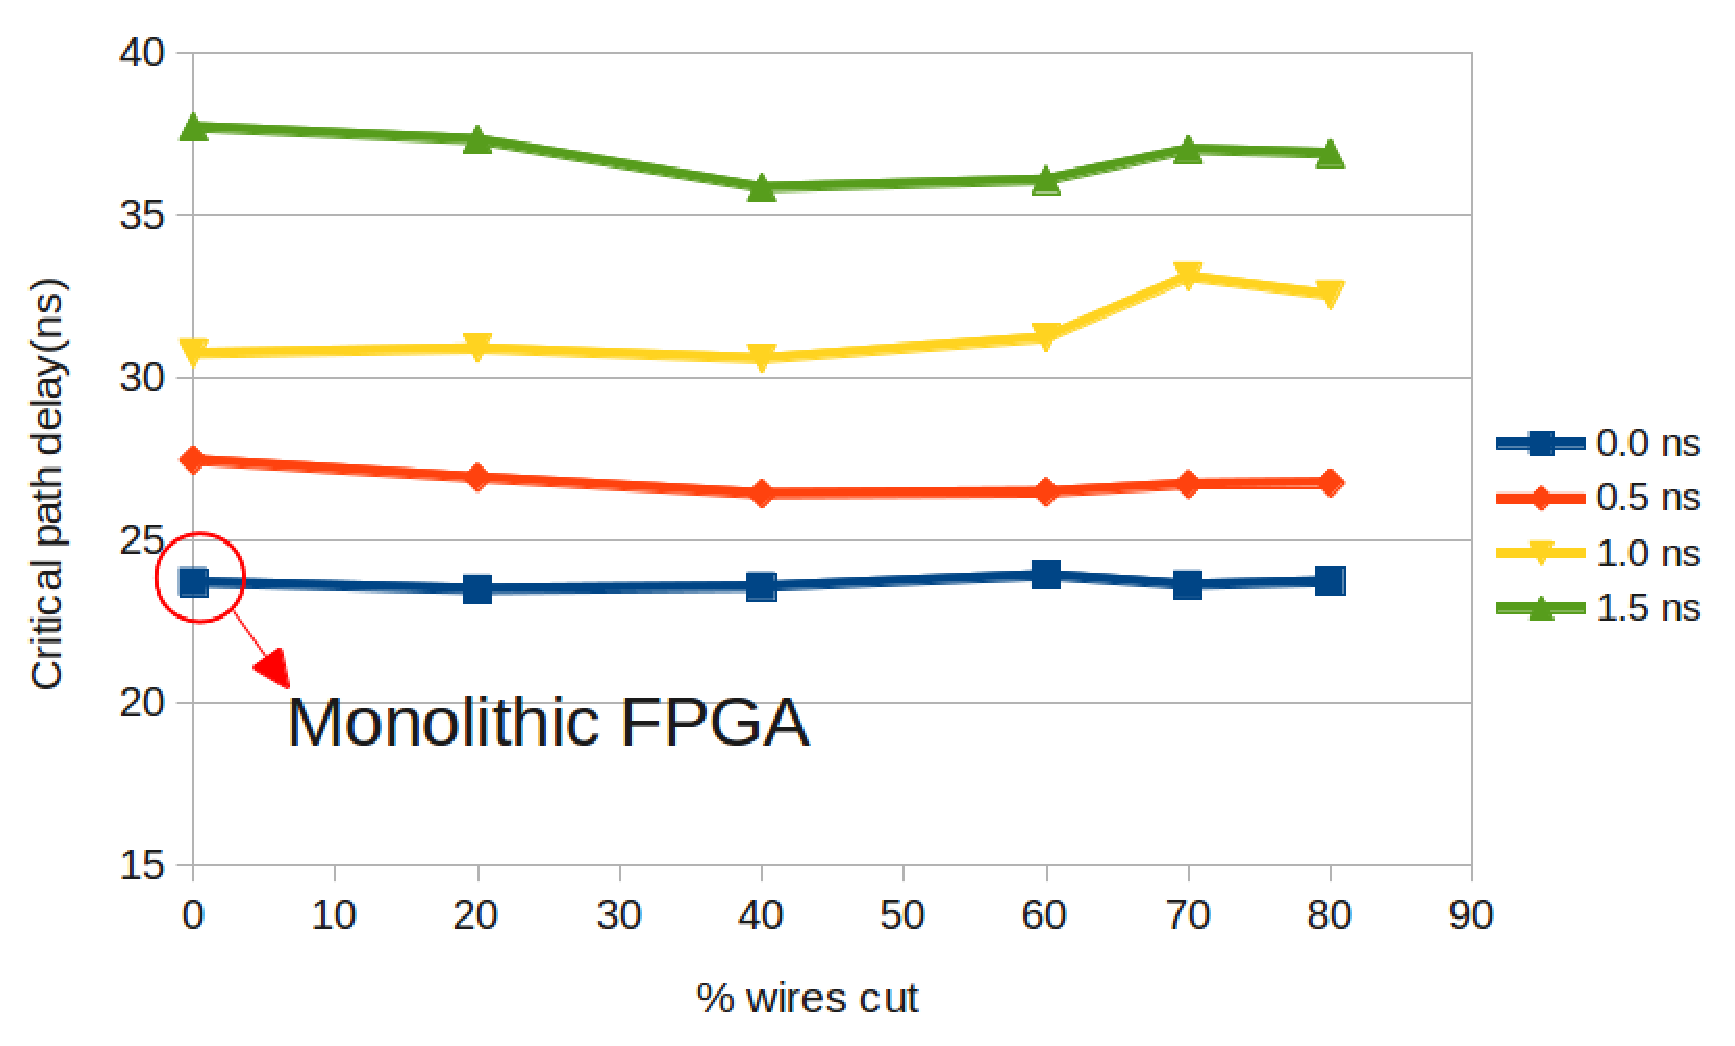
\includegraphics[width=\linewidth]{delays_crit_path.eps}
\caption{Critical path delay vs. \textit{\% wires cut} for 3 cuts and $0.0$, $0.5$, $1.0$ and $1.5ns$ of \textit{delay increase}.}
\label{fig:delays_crit}
\end{figure}

\begin{table}[!htbp]
\begin{tabular}{|l|r|r|r|r|r|r|}
\hline
\% wires cut & 0 & 20 & 40 & 60 & 70 & 80 \\ \hline  \hline
bgm & 25.9 & 26.3 & 25.8 & 26.1 & 25.8 & 26.7 \\ \hline
LU32PEEng & 113 & 113 & 117 & 118 & 113 & 114 \\ \hline
LU8PEEng & 115 & 114 & 116 & 115 & 118 & 115 \\ \hline
mcml & 77.2 & 78.7 & 79.5 & 80.5 & 77.3 & 76.7 \\ \hline
mkDelayWorker32B & 7.8 & 7.6 & 7.5 & 7.7 & 7.5 & 7.6 \\ \hline
stereovision0 & 4.5 & 4.3 & 4.5 & 4.5 & 4.5 & 4.5 \\ \hline
stereovision1 & 6.0 & 6.2 & 5.9 & 6.3 & 6.2 & 6.2 \\ \hline
stereovision2 & 18.0 & 17.1 & 17.1 & 17.5 & 17.6 & 17.7 \\ \hline
Geometric mean & 23.7 & 23.5 & 23.6 & 23.9 & 23.6 & 23.7 \\ \hline
\end{tabular}
\caption{Critical path delay (in \textit{ns}) when \textit{number of cuts = 3} and \textit{increased delay = 0ns}.}
\label{table:delay0}
\end{table}

\begin{table}[!htbp]
\begin{tabular}{|l|r|r|r|r|r|r|}
\hline
\% wires cut & 0 & 20 & 40 & 60 & 70 & 80 \\ \hline \hline
bgm & 31.6 & 30.3 & 29.2 & 29.2 & 29.9 & 31.6 \\ \hline
LU32PEEng & 119 & 114 & 115 & 114 & 115 & 115 \\ \hline
LU8PEEng & 118 & 116 & 119 & 117 & 114 & 115 \\ \hline
mcml & 82.6 & 82.7 & 79.6 & 81.9 & 84.5 & 82.6 \\ \hline
mkDelayWorker32B & 9.8 & 10.6 & 10.4 & 9.6 & 10.2 & 9.1 \\ \hline
stereovision0 & 5.7 & 5.3 & 4.8 & 4.9 & 4.9 & 4.8 \\ \hline
stereovision1 & 8.0 & 7.5 & 7.4 & 8.2 & 7.9 & 8.0 \\ \hline
stereovision2 & 20.1 & 19.7 & 20.3 & 19.9 & 20.2 & 21.6 \\ \hline
Geometric mean & 27.5 & 26.9 & 26.4 & 26.5 & 26.7 & 26.8 \\ \hline
\end{tabular}
\caption{Critical path delay (in \textit{ns}) when \textit{number of cuts = 3} and \textit{increased delay = 0.5ns}.}
\label{table:delay500}
\end{table}

\begin{table}[!htbp]
\begin{tabular}{|l|r|r|r|r|r|r|}
\hline
\% wires cut & 0 & 20 & 40 & 60 & 70 & 80 \\ \hline \hline
bgm & 47.2 & 52.4 & 43.1 & 42.7 & 44.8 & 48.3 \\ \hline
LU32PEEng & 115 & 112 & 117 & 114 & 116 & 113 \\ \hline
LU8PEEng & 161 & 159 & 122 & 146 & 118 & 129 \\ \hline
mcml & 94.0 & 86.0 & 93.9 & 88.7 & 77.3 & 87.5 \\ \hline
mkDelayWorker32B & 15.3 & 13.8 & 14.3 & 15.3 & 17.9 & 15.4 \\ \hline
stereovision0 & 7.5 & 9.4 & 8.9 & 7.8 & 9.6 & 8.3 \\ \hline
stereovision1 & 14.6 & 12.0 & 13.1 & 12.7 & 14.6 & 14.8 \\ \hline
stereovision2 & 29.9 & 30.3 & 28.7 & 30.3 & 30.1 & 29.8 \\ \hline
Geometric mean & 37.7 & 37.3 & 35.9 & 36.1 & 37.0 & 36.9 \\ \hline
\end{tabular}
\caption{Critical path delay (in \textit{ns}) when \textit{number of cuts = 3} and \textit{increased delay = 1.5ns}.}
\label{table:delay1500}
\end{table}


%   - Impact of # of cutlines
\subsection{Impact of Number of Dice}

To examine the impact of the number of die used to construct an interposer-based FPGA, we varied the number of cuts from 1 to 3 (which varies the number of die from 2 to 4).  In these experiments, the \textit{delay increase} was kept constant at $1ns$. 

As shown in Figure \ref{fig:cuts_minW}, the number of cuts does have an impact on the minimum channel width, but not a very large or constant one. At 80\% of wires cut the experiments with 2 and 3 cuts had the minimum channel width only 8\% and 10\%, respectively, greater than the scenario with only 1 cut. At lower values of \textit{\% wires cut} the difference was even smaller.

Figure \ref{fig:cuts_crit} shows that the number of dice in an interposer-based FPGA impacts circuit speed significantly, as the critical path delay rises significantly as systems have more cuts. Recall that a monolithic FPGA has a geometric average critical path delay of $23.7ns$ for our test architecture. With \textit{number of cuts} $= 1$ the critical path delay increases by 3 to 4 ns, while with \textit{number of cuts} $= 2$ the critical path delay increases by 5 to 6 ns. With \textit{number of cuts} $= 3$, the critical path delay is typically 7 ns higher than that of a monolithic FPGA.

Tables \ref{table:1cut_minW}, \ref{table:1cut_path}, \ref{table:2cut_minW}, \ref{table:2cut_path}, \ref{table:standard_minW} and \ref{table:standard_path} show the minimum channel width and critical path delay for each circuit for each of the different scenarios. The critical path results for individual circuits again follow the overall averages well. Some of the minimum channel widths for individual circuits show anomalous trends as the number of cutlines increase, however. For example, \textit{mcml} often has a smaller minimum channel width with 2 cuts than with 1 cut. This may be due to a circuit structure that leads to easier division into thirds than halves, but also likely indicates room for further CAD optimization.

\begin{figure}[!htbp]
\centering
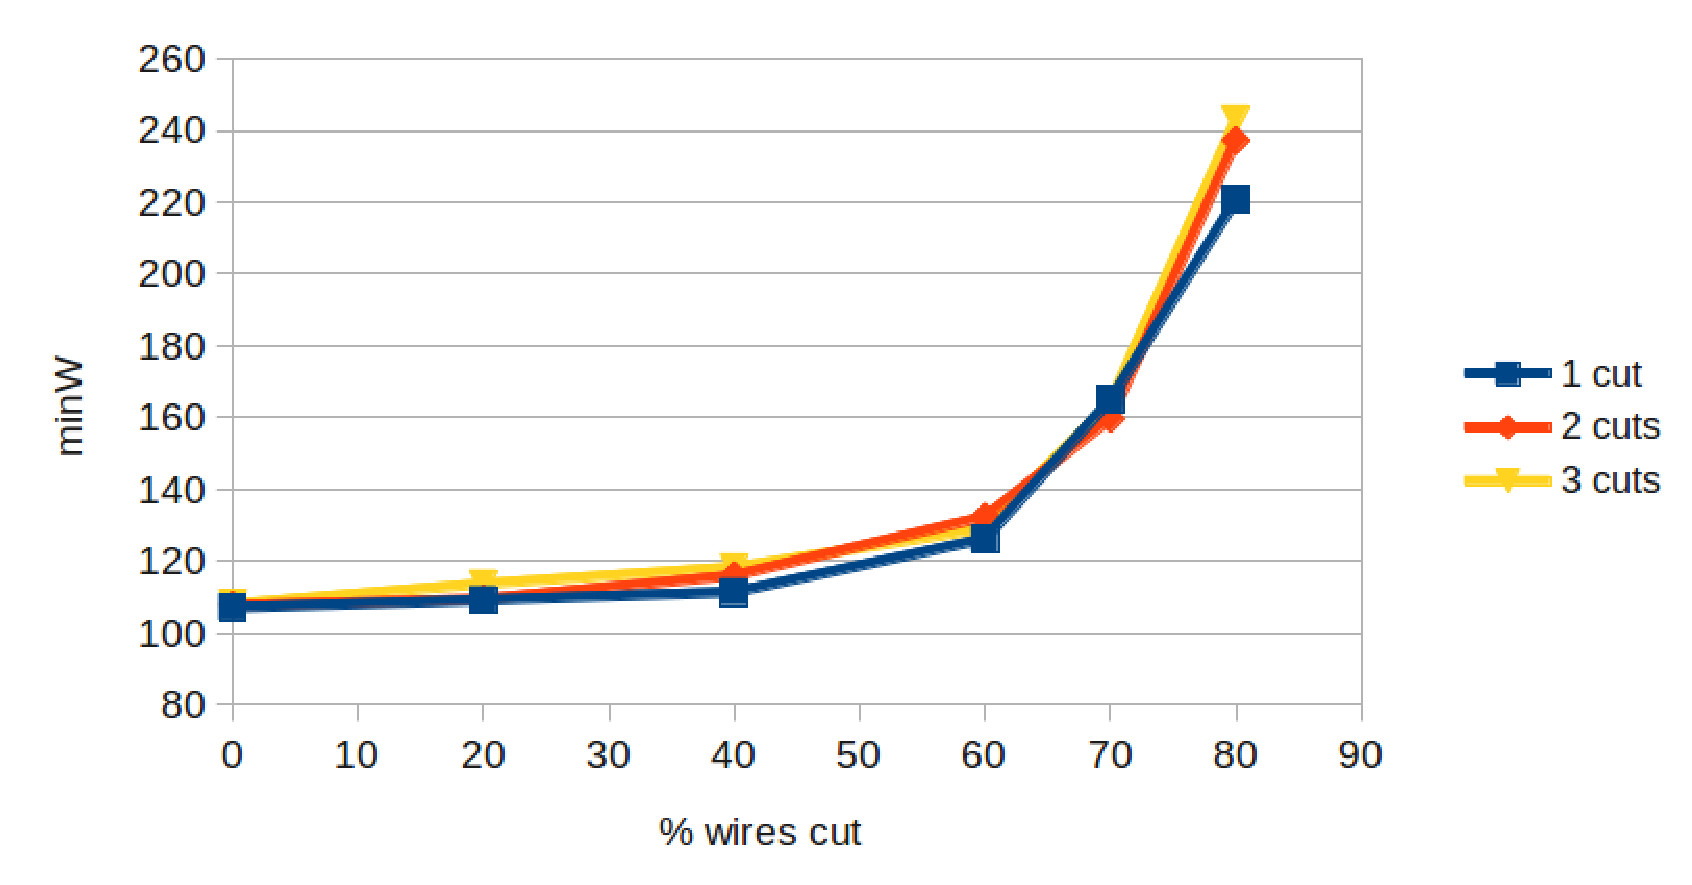
\includegraphics[width=\linewidth]{cuts_minW.eps}
\caption{Minimum channel width vs. \textit{\% wires cut} for 1, 2 and 3 cuts and $1ns$ of \textit{delay increase}.}
\label{fig:cuts_minW}
\end{figure}

\begin{figure}[!htbp]
\centering
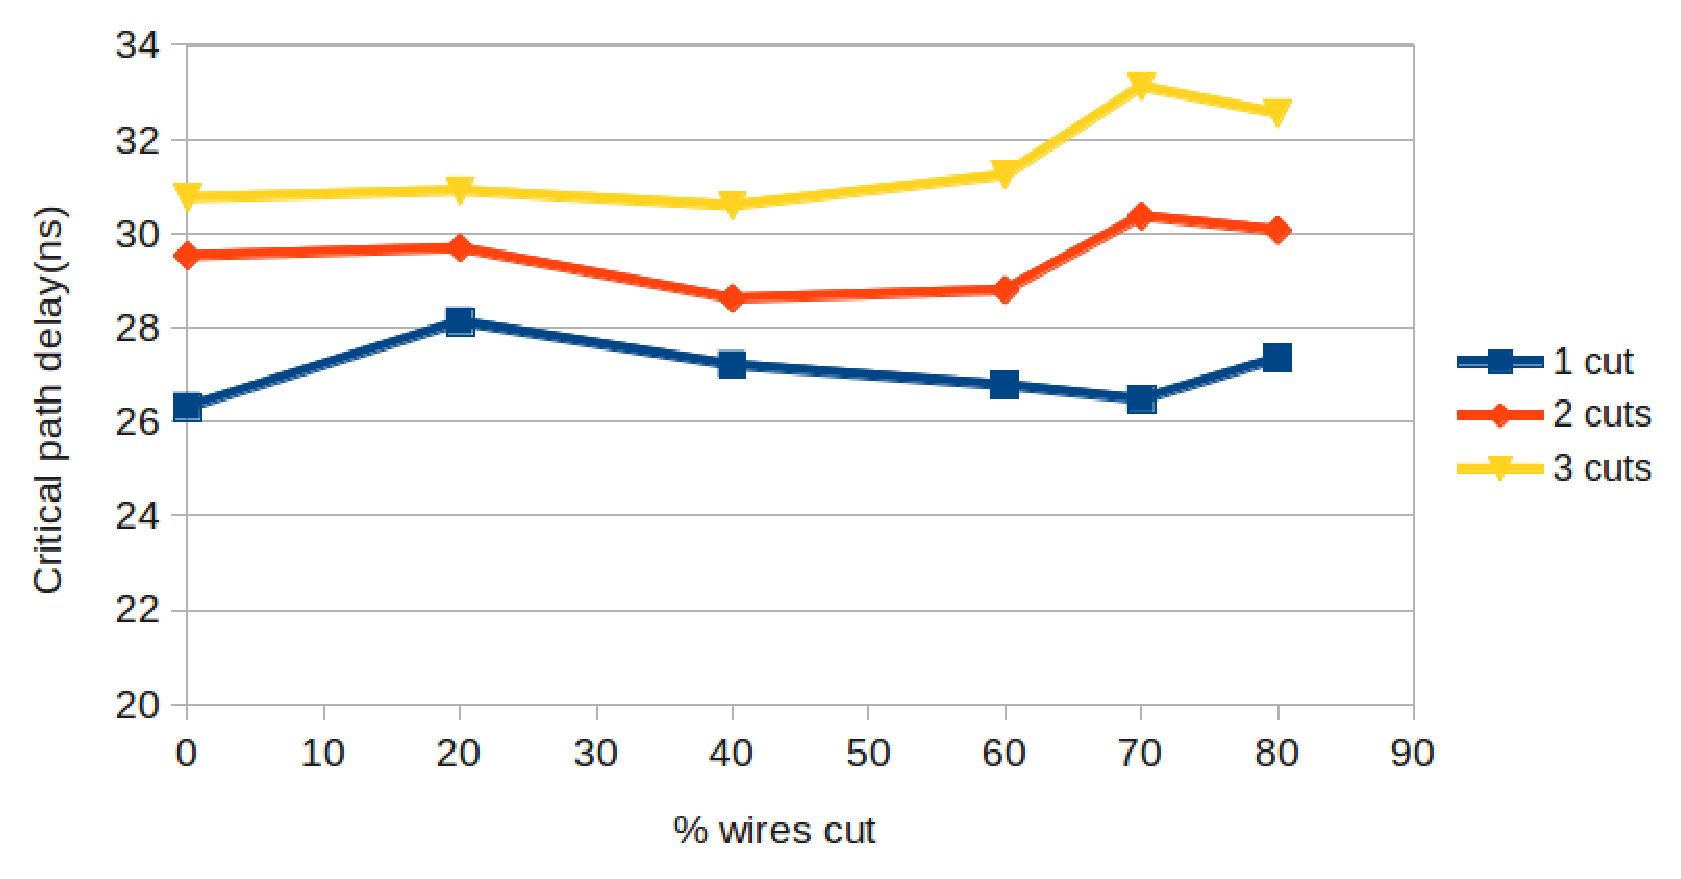
\includegraphics[width=\linewidth]{cuts_crit_path.eps}
\caption{Critical path delay vs. \textit{\% wires cut} for 1, 2 and 3 cuts and $1ns$ of \textit{delay increase}.}
\label{fig:cuts_crit}
\end{figure}

\begin{table}[!htbp]
\begin{tabular}{|l|r|r|r|r|r|r|}
\hline
\% wires cut & 0 & 20 & 40 & 60 & 70 & 80 \\ \hline \hline
bgm & 114 & 114 & 122 & 126 & 142 & 156 \\ \hline
LU32PEEng & 170 & 176 & 182 & 206 & 318 & 396 \\ \hline
LU8PEEng & 110 & 114 & 116 & 138 & 164 & 236 \\ \hline
mcml & 108 & 114 & 106 & 124 & 150 & 238 \\ \hline
mkDelayWorker32B & 74 & 78 & 80 & 88 & 98 & 138 \\ \hline
stereovision0 & 62 & 60 & 62 & 76 & 132 & 146 \\ \hline
stereovision1 & 102 & 104 & 106 & 108 & 144 & 186 \\ \hline
stereovision2 & 160 & 158 & 164 & 200 & 264 & 432 \\ \hline
Geometric mean & 107 & 109 & 111 & 126 & 165 & 221 \\ \hline
\end{tabular}
\caption{Minimum channel width when \textit{number of cuts = 1} and \textit{increased delay = 1ns}.}
\label{table:1cut_minW}
\end{table}

\begin{table}[!htbp]
\begin{tabular}{|l|r|r|r|r|r|r|}
\hline
\% wires cut & 0 & 20 & 40 & 60 & 70 & 80 \\ \hline \hline
bgm & 26.5 & 32.1 & 28.3 & 30.2 & 27.5 & 30.0 \\ \hline
LU32PEEng & 113 & 113 & 113 & 115 & 114 & 111 \\ \hline
LU8PEEng & 117 & 118 & 116 & 114 & 114 & 116 \\ \hline
mcml & 82.5 & 82.0 & 83.0 & 84.5 & 83.2 & 77.9 \\ \hline
mkDelayWorker32B & 11.2 & 11.4 & 11.2 & 9.9 & 10.6 & 11.5 \\ \hline
stereovision0 & 4.5 & 5.1 & 5.0 & 4.9 & 4.9 & 5.4 \\ \hline
stereovision1 & 7.4 & 8.2 & 8.4 & 7.2 & 7.2 & 7.9 \\ \hline
stereovision2 & 21.3 & 23.1 & 20.9 & 22.3 & 21.6 & 20.9 \\ \hline
Geometric mean & 26.3 & 28.1 & 27.2 & 26.8 & 26.5 & 27.3 \\ \hline
\end{tabular}
\caption{Critical path delay (in \textit{ns}) when \textit{number of cuts = 1} and \textit{increased delay = 1ns}.}
\label{table:1cut_path}
\end{table}

\begin{table}[!htbp]
\begin{tabular}{|l|r|r|r|r|r|r|}
\hline
\% wires cut & 0 & 20 & 40 & 60 & 70 & 80 \\ \hline \hline
bgm & 114 & 116 & 130 & 140 & 172 & 272 \\ \hline
LU32PEEng & 170 & 180 & 186 & 198 & 264 & 426 \\ \hline
LU8PEEng & 110 & 114 & 116 & 124 & 158 & 246 \\ \hline
mcml & 108 & 110 & 126 & 138 & 114 & 150 \\ \hline
mkDelayWorker32B & 76 & 80 & 82 & 88 & 100 & 132 \\ \hline
stereovision0 & 62 & 58 & 60 & 88 & 114 & 166 \\ \hline
stereovision1 & 104 & 108 & 116 & 136 & 184 & 296 \\ \hline
stereovision2 & 160 & 156 & 162 & 188 & 246 & 362 \\ \hline
Geometric mean & 108 & 109 & 116 & 132 & 160 & 237 \\ \hline
\end{tabular}
\caption{Minimum channel width when \textit{number of cuts = 2} and \textit{increased delay = 1ns}.}
\label{table:2cut_minW}
\end{table}

\begin{table}[!htbp]
\begin{tabular}{|l|r|r|r|r|r|r|}
\hline
\% wires cut & 0 & 20 & 40 & 60 & 70 & 80 \\ \hline \hline
bgm & 31.0 & 30.3 & 28.3 & 36.1 & 35.9 & 37.5 \\ \hline
LU32PEEng & 113 & 113 & 119 & 113 & 117 & 112 \\ \hline
LU8PEEng & 118 & 118 & 117 & 116 & 118 & 114 \\ \hline
mcml & 82.9 & 86.3 & 81.3 & 80.9 & 82.4 & 82.8 \\ \hline
mkDelayWorker32B & 12.3 & 12.1 & 9.8 & 11.1 & 13.5 & 11.3 \\ \hline
stereovision0 & 6.4 & 5.7 & 6.3 & 5.3 & 5.3 & 5.9 \\ \hline
stereovision1 & 9.3 & 10.4 & 9.5 & 9.6 & 10.2 & 9.9 \\ \hline
stereovision2 & 22.9 & 24.2 & 24.0 & 21.6 & 24.2 & 25.5 \\ \hline
Geometric mean & 29.5 & 29.7 & 28.6 & 28.8 & 30.4 & 30.1 \\ \hline
\end{tabular}
\caption{Critical path delay (in \textit{ns}) when \textit{number of cuts = 2} and \textit{increased delay = 1ns}.}
\label{table:2cut_path}
\end{table}

\section{Conclusions and Future Work}
\label{conclusionSection}

We have extended VPR to model and optimize for interposer-based multi-FPGA systems. While such systems are now a commercial reality, we do not know of any prior study of their key architectural parameters. We found that by modifying VPR's placement cost function we could improve the routability (reduce minW) by 18\%, while simultaneously improving speed by 2\%. Interestingly, we found that a smooth cost function that less precisely models the interposing wiring demand outperformed direct monitoring of the number of required interposer connections during annealing.

We defined three key architecture parameters for interposer-based FPGAs, and used this extended VPR to analyze their impact on minimum channel width and critical path delay. We found that the \textit{minimum channel width} increases steeply after more than 60\% of the within-die wires are cut at the interposer, and when 80\% of wires are cut the \textit{minimum channel width} is more than double that required by a monolithic FPGA. The Xilinx \textit{XC7V2000T} FPGA has 77\% of the normal wiring cut at the interposer, indicating that commercial interposer-based FPGAs will require high-quality CAD optimization to maintain good routability. The \textit{critical path delay} is not strongly influenced by the \textit{\% wires cut} but is strongly influenced by the interposer delay and the number of cuts. Our results show that the critical path usually crosses the interposer cutline more than once, as the \textit{critical path delay} is increased by more than the interposer \textit{delay increase}. Increasing the number of dice in an interposer-based FPGA does not significantly impact the \textit{minimum channel width}, but does lead to a larger \textit{critical path delay}.

There are many interesting CAD and architecture questions for interposer-based FPGAs which we plan to investigate.  Currently the wires that cross the interposer are accessed with the same switch structure as other wires in the FPGA. Since interposer wires are more scarce, possibly these wires should have larger multiplexers feeding them, which would make them easier to use; this may help routability of the system. Such changes will have to be carefully considered however, to make sure the FPGA can still be laid out as an array of regular tiles. Alternative CAD flows to improve the interposer routability are also possible. For example, instead of following the synthesize, place and route CAD flow of a conventional FPGA, we could add a partitioning step before placement which would divide the circuit into one partition per die. Such a flow may improve routability, as a partitioner's main focus is minimizing the number of cut signals. Enhanced partitioners will be required, as current partitioners such as hMetis~\cite{hMetis} cannot model the heterogeneous balance constraint (i.e. use no more than the available device logic, RAM, DSP and I/O blocks in any die) present in FPGAs. Additionally, by dividing the placement problem into two pieces -- partitioning and within-die placement -- we may increase the critical path delay as we can no longer globally optimize the placement of timing critical paths in one unified placement step. Nonetheless, this is a viable alternative approach and a comparison to the approach taken in this paper would be very interesting.

%ACKNOWLEDGMENTS are optional
\section{Acknowledgments}

This work was supported by a Ci\^{e}ncia sem Fronteiras scholarship from CNPq - Brazil and the NSERC/Altera Industrial Research Chair in Programmable Silicon.
%
\bibliographystyle{abbrv}
\bibliography{fpga2014paper}

\balancecolumns
% That's all folks!
\end{document}
